\documentclass[twoside,11pt]{article}

\usepackage[abbrvbib, preprint]{jmlr2e}

\usepackage{amsmath,amsfonts,setspace,natbib,amssymb,ifthen,url,array,color,hyperref}

\newcommand{\x}{\mathbf{x}}
\newcommand{\LL}{\mathbf{L}}
\newcommand{\TE}{\mathrm{TE}}
\newcommand{\E}{\mathbb{E}}
\newcommand{\distance}{\mathrm{distance}}
\newcommand{\MG}{\mathrm{MG}}
\newcommand{\tr}{\textrm{tr}}
\newcommand{\KNN}{\textrm{KNN}}
\newcommand{\malts}{\textsc{MALTS}}
\newcommand{\dis}{\mathbf{d}}
\newtheorem{define}{Definition}
\newcommand{\todo}[1]{{\color{red}\emph{xx #1 xx}}}
\DeclareMathOperator*{\argmax}{arg\,max}
\DeclareMathOperator*{\argmin}{arg\,min}
              
\newcommand{\indep}{\rotatebox[origin=c]{90}{$\models$}}

\definecolor{brown}{rgb}{0.8,0.1,0.1}
\definecolor{BROWN}{rgb}{0.8,0.1,0.1}
\definecolor{red}{rgb}{1,0,0}
\definecolor{RED}{rgb}{1,0,0}
\newcommand{\ques}[1]{{\bfseries #1}}
\newcommand{\ans}[1]{{\textbf{Ans.}~~#1}}
\newcommand{\reva}[1]{{{\color{burntumber}{#1}}}}
\newcommand{\revb}[1]{{{\color{blue}{#1}}}}
\newcommand{\revc}[1]{{{\color{magenta}{#1}}}}
\definecolor{dartmouthgreen}{rgb}{0.05, 0.5, 0.06}
\definecolor{burntumber}{rgb}{0.54, 0.2, 0.14}
\definecolor{BURNTUMBER}{rgb}{0.54, 0.2, 0.14}
\newcommand{\revd}[1]{{{\color{dartmouthgreen}{#1}}}}
\newcommand{\revm}[1]{{{\color{red}{#1}}}}


 

\bibpunct[, ]{(}{)}{,}{a}{}{,}%
\def\bibfont{\small}%
\def\bibsep{\smallskipamount}%
\def\bibhang{24pt}%
\def\newblock{\ }%
\def\BIBand{and}%


\renewcommand{\bibname}{References}
\renewcommand{\bibsection}{\subsubsection*{\bibname}}

\usepackage{bbm}
\usepackage{lscape}


\jmlrheading{1}{2019}{0-0}{0/00}{0/00}{harsh1234}{Harsh Parikh, Cynthia Rudin and Alexander Volfovsky}

\ShortHeadings{MALTS}{Parikh, Rudin and Volfovsky}

\firstpageno{1}

\title{MALTS: Matching After Learning to Stretch}
	
    \author{\name Harsh Parikh \email           harsh.parikh@duke.edu \\
        \addr Department of Computer Science\\
        Duke University\\
        Durham, NC 27708-0129, USA.
        \AND
        \name Cynthia Rudin \email cynthia@cs.duke.edu \\
        \addr Department of Computer Science\\
        Duke University\\
        Durham, NC 27708-0129, USA.
        \AND
        \name Alexander Volfovsky \email alexander.volfovsky@duke.edu\\
        \addr Department of Statistical Science\\
        Duke University\\
        Durham, NC 27710, USA.
     }

\begin{document}
	
  	\maketitle

    \begin{abstract}
		We introduce a flexible framework that produces high-quality almost-exact matches for causal inference. Most prior work in matching uses ad-hoc distance metrics, often leading to poor quality matches, particularly when there are irrelevant covariates. In this work, we learn an interpretable distance metric for matching, which leads to substantially higher quality matches. The learned distance metric stretches the covariates according to their contribution to outcome prediction.
        The framework is flexible in that the user can choose the form of the distance metric and the type of optimization algorithm. Our ability to learn flexible distance metrics leads to matches that are interpretable and useful for the estimation of conditional average treatment effects.
	\end{abstract}

\begin{keywords}
  causal inference, matching, nearest neighbor, distance metric learning
\end{keywords}
	\allowdisplaybreaks
	%!TEX root = main.tex
\section{Introduction}
Matching methods are used throughout the social and health sciences to make causal conclusions where access to randomized trials is scarce but observational data are widely available. 
Matching methods construct groups of similar individuals, some of whom select into treatment and some of whom select into control, allowing for direct comparison of outcomes between these populations. Matching methods are particularly interpretable since they allow fine-grained troubleshooting of the data. 
For instance, examining the matched groups may allow the user to detect unmeasured confounding that led some units to have a higher chance of being treated or a higher chance of leading to a positive outcome.
Having high-quality matches also allows the user to estimate nonlinear treatment effects with lower bias than parametric approaches.
The quality of the matches is our main consideration in this work.

Typically, matching methods place units that are close together into the same matched group, where closeness is measured in terms of a pre-defined distance (e.g., exact, coarsened exact, Euclidean, etc.), while maintaining balance constraints between treatment and control units. Despite its merits, this classical paradigm has flaws, namely that it relies heavily on a prespecified distance metric. The distance metric cannot be determined without an understanding of the importance of the variables;
for instance, the quality of matches for any prespecified distance weighing all covariates equally will degrade as the number of irrelevant covariates increases. 
This is true irrespective of the matching methodology employed.
This has previously been referred to as the toenail problem \citep{wang2017flame, DiengEtAl2018}, where the inclusion of irrelevant covariates (like toenail length) with nonzero weights can overwhelm the metric for matching. A related concern is that the covariates may be scaled differently, where a given distance along one covariate has a different impact than the same distance along a different covariate; in this case, if the weights on the covariates are chosen poorly, the total distance metric can inadvertently be determined by less relevant covariates, again leading to lower quality matches.

Ideally, the distance metric would capture important covariates that significantly contribute in generating the outcome, so that after matching, treatment effect estimates computed within the matched groups would be accurate estimates of treatment effects. If the researcher knows how to choose the distance metric so that it yields accurate treatment effect estimates, this would solve the problem. However, there is no reason to believe that this is achievable in high-dimensional and complex data settings. Producing high dimensional functions to characterize data is a task at which humans are not naturally adept.

In this work, we propose a framework for matching where an interpretable distance measure between matched units is learned from a held-out training set. As long as the distance metric generalizes from the training set to the full sample, we are able to compute high-quality matches and accurate estimates of conditional average treatment effects (CATEs) within the matched groups. One can use any form of distance metric to train, and in this work, we focus on exact matching for discrete variables and generalized Mahalanobis distances for continuous variables. By definition, the generalized Mahalanobis distance is determined by a matrix. If the matrix is diagonal, the distance calculation represents a stretch for each covariate. Irrelevant covariates will be compressed so that their values are always effectively zero. Highly relevant covariates will be stretched so that for two units to be considered a match, they must have very similar values for those covariates. In this way, diagonal matrices lead to very interpretable distance metrics. If the Mahalanobis distance matrix is not constrained to be diagonal, then it induces a stretch and rotation, leading to more flexible but less interpretable notions of distance. 

The new framework is called Learning-to-Match, and the algorithm introduced in this work is called Matching After Learning to Stretch (MALTS). We tested MALTS against several other matching methods in simulation studies, where ground truth CATEs are known. In these experiments, MALTS achieves substantially and consistently better results than other matching methods including Genmatch, propensity score matching, and standard (non-learned) Mahalanobis distance in estimating CATEs. Even though our method is heavily constrained to produce interpretable matches, it performs at the same level as non-matching methods that are designed to fit extremely flexible but uninterpretable models directly to the response surface.

%We use MALTS to study the effect of a large drug treatment program (Breaking the Cycle - BTC  \cite{}) on crime reduction, which is relevant to the current opioid epidemic. We find that the important covariates for matching in the BTC drug treatment program are ???, and we identify subgroups for which there is a (heterogeneous) treatment effect.
	% !TEX root = main.tex
\section{Related work}

Since the 1970's, the causal inference literature on matching methods has been concentrated on dimension reduction techniques \citep[e.g.,][]{rubin1973matching,rubin1973use,rubin1976multivariate,cochran1973controlling}. In this literature, the leading approach for dimension reduction uses the propensity score, the conditional probability of treatment given covariate information.
Propensity score methods target average treatment effects and so do not produce exact matches or almost-exact matches. When treatment is binary, they project data onto one dimension, and closeness of units in propensity score does not imply their closeness in covariate space. As a result, the matches cannot directly be used for estimating heterogeneous treatment effects. Fast and flexible matching methods have been studied in the literature to estimate average treatment effects because fully efficient matching might be computationally inefficient \citep{gu1993, imbens2004nonparametric}. However, these method are often ineffective in producing high quality CATE estimates. Regression methods can be used for CATE estimation, but this assumes that the regression method is correctly specified -- or in the case of doubly robust estimation \citep[e.g., ][]{farrell2015robust}, either the propensity model or the outcome model needs to be correctly specified. 
Machine learning approaches generalize regression approaches and can create models that are extremely flexible and predict outcomes accurately for both treatment and control groups \citep{hill2011bayesian,chernozhukov2016double,hahn2017bayesian}. However, complicated regression methods lose the interpretability inherent to almost-exact matches.
%Analogously,  again leading to a sacrifice in interpretability.
 In practice, MALTS performs similarly to (or better than) several machine learning methods in our experiments, despite being restricted to interpretable almost-exact matches with an interpretable distance metric.

A flexible setup for producing high-quality matches is provided by the optimal matching literature \citep{rosenbaum2016imposing}. These are built on network flow algorithms and integer programming to produce matches that are constrained in user-defined ways \citep{zubizarreta2012using,zubizarreta2014matching,keele2014optimal,resa2016evaluation,AlamRu15,AlamRu15nonparam,pmlr-v54-kallus17a}. In all of these approaches, the user defines the distance metric rather than learning it through data, which is time-consuming and likely inaccurate, potentially leading to poor quality of the matched groups. 

An alternative to optimal matching is coarsened exact matching (CEM) \citep{iacus2012causal}, an approach that requires users to specify explicit bins for all covariates on which to construct matches. 
This requires users to know in advance that the outcomes are insensitive to movements within many high-dimensional bins, 
which is essentially equivalent to the user knowing the answer to the problem we investigate in this work. Large amounts of user choice to define these bins can also lead to unintentional user bias. By \textit{learning} the stretching rather than asking the user to define it as in CEM, this bias is potentially reduced. 
Alternatively, \cite{zhao2004} and \cite{imbens2004nonparametric} discusses the choice of distance metric for matching. The approach by \cite{zhao2004} depends on the correlations between treatment choice, outcome and covariates. However, this approach assumes a model for the relationship between the outcome and covariates, or the treatment choice and covariates. Hence, under model misspecification, the estimator may not be consistent. MALTS learns a distance metric without any model assumptions. 
The present work builds on work of  \cite{wang2017flame, DiengEtAl2018} where a discrete distance metric is learned by considering the prediction quality of the covariate sets. 

There is substantial work on learning distance metrics \citep[e.g.,][]{goldberger2005neighbourhood,weinberger2006distance,weinberger2009distance}, where the goal is to learn a distance metric in latent space to separate different classes of data in supervised learning, often with a margin. This is different from our goal of matching for causal inference, but some of our proofs were inspired by this work in supervised learning. 

MALTS was used for the Atlantic Causal Inference Competition \citep{harsh2019acic}.
	\section{Learning-to-Match Framework}\label{sec:framework}
Within this framework, we perform treatment effect estimation using following three stages: 1) learning a distance metric, 2) matching samples, and 3) estimating CATEs. 

We denote the $p$ dimensional covariate vector space as $\mathcal{X}\subset \mathbb{R}^p$ and the unidimensional outcome space by $\mathcal{Y} \subset \mathbb{R}$. Let $\mathcal{T}$ be a finite label set of treatment indicators (in this paper we consider only the binary case). Let $\mathcal{Z}=\mathcal{X}\times\mathcal{Y}\times\mathcal{T}$ such that $z=(\x,y,t)\in \mathcal{Z}$ means that $\x\in\mathcal{X}$, $y\in\mathcal{Y}$ and $t\in\mathcal{T}$. Let $\mu$ be an unknown probability distribution over $\mathcal{Z}$ such that $\forall z \in \mathcal{Z}, ~ \mu(z)>0$. We assume that $\mathcal{X}$ is a compact convex space with respect to $\|\cdot\|_2$, thus there exists a constant $\mathbf{C}_x$ such that $\|\x\|_2\leq\mathbf{C}_x$. Also, $|y|\leq\mathbf{C}_y$. A distance metric is a symmetric, positive definite function with two arguments from $\mathcal{X}$ such that $\dis: \mathcal{X}\times\mathcal{X} \to \mathbb{R}^+$. A distance metric must obey the triangle inequality. Let $\mathcal{S}_n$ denote a set of $n$ observed units $\{s_1,...,s_n\}$ drawn i.i.d. from $\mu$ such that $\forall i, ~s_i \in \mathcal{Z}$. We parameterize $\dis$ with parameter $\mathcal{M}(\cdot)$, explicitly calling it $\dis_\mathcal{M}$, and let $\mathcal{M}(\mathcal{S}_n)$ denote the parameter learned using $\textsc{MALTS}$ methodology which is described in Section~\ref{sec:method}. 
For ease of notation, we will denote the observed sample of treated units as $\mathcal{S}^{(T)}_n := \{s^{(T)}_i = (\x_i,y_i,t_i)~|~ s^{(T)}_i \in \mathcal{S}_n \text{ and } t_i = T \}$ and the observed sample of control units as $\mathcal{S}^{(C)}_n := \{s^{(C)}_i = (\x_i,y_i,t_i)~|~ s^{(C)}_i \in \mathcal{S}_n \text{ and } t_i = C \}$.
We assume no unobserved confounders and standard ignorability assumptions, i.e.  $\forall i,~ (Y^{(T)},Y^{(C)})~ \indep ~T ~|~ (X=\x_i)$ \citep{Rubin2005}. For each individual unit $s_i = (\x_i,y_i,t_i) \in \mathcal{Z}$ we define its conditional average treatment effect (or individualized treatment effect) as the difference of potential outcomes of unit $i$ under the treatment and control, $\tau(\x_i) = \mathbbm{E}\left[Y^{(T)} - Y^{(C)} | X=\x_i \right] = y^{(T)}(\x_i) -y^{(C)}(\x_i)$. For notational simplicity we sometimes refer $y^{(T)}(\x_i)$ as $y^{(T)}_i$ and $y^{(C)}(\x_i)$ as $y^{(C)}_i$ We use the $\;\widehat{}$ (hat) notation to refer to estimated values. 
%using the given covariate vector.
% In our framework, a learning-to-match algorithm consist of three modeling decisions: the form of distance metric used for matching, the method of learning parameters of that distance metric, and the method of matching. 
%A training set is used to train the parameters of the distance metric, and that learned distance metric is used on the rest of the sample in the test-set for matching and CATE prediction. 


Our goal is to minimize the expected loss between estimated treatment effects $\widehat{\tau}(\x)$ and true treatment effects $\tau(\x)$ across target population $\mu(z)$ (this can either be a finite or super-population).

Let the population expected loss be:
\begin{eqnarray*}
\E\left[ \ell(\widehat{\tau}(\x),\tau(\x))\right]
=
\int \ell(\widehat{\tau}(\x),\tau(\x))d\mu
=
\int \ell(\hat{y}^{(T)}(\x)-\hat{y}^{(C)}(\x), {y}^{(T)}(\x)-{y}^{(C)}(\x)) d\mu.
\end{eqnarray*}
% \todo{should this expectation be over X or over X and T?}
We use absolute loss, $\ell(a,b)=|a-b|$. 
For a finite random i.i.d$.$ sample $\{s_i=(\x_i,y_i,t_i)\}^n_{i=1}$ from the distribution $\mu$, we could estimate the sample average loss as 
\begin{eqnarray*}
% \E \ell(\widehat{\tau}(\x),\tau(\x))
% \approx
\frac{1}{n}\sum_{i=1}^n \ell(\hat{y}^{(T)}(\x_i)-\hat{y}^{(C)}(\x_i), {y}^{(T)}(\x_i)-{y}^{(C)}(\x_i)),
\end{eqnarray*}
where $y^{(T)}(\x_i)$ and $y^{(C)}(\x_i)$ are the counterfactual outcome values for the units in the sample $\{s_i=(\x_i,y_i,t_i):i=1,\dots,n\}$.
However, the difficulty in causal inference is that we only observe treatment outcomes $y^{(T)}(\x_i)$ or control outcomes $y^{(C)}(\x_i)$ for an individual $i$ in the sample. Hence, we cannot directly calculate the treatment effect for any individual. For units in the treatment set we know $y^{(T)}(\x_i)$ and so we replace $\hat{y}^{(T)}(\x_i)$ by $y^{(T)}(\x_i)$, and analogously for units in the control set. Thus breaking the sum into treatment and control group:
\begin{eqnarray*}
% \E_{\mu} \ell(\widehat{\tau}(\x),\tau(\x))
% \approx&
\frac{1}{n_t}
\sum_{i \in \textrm{treated}} \ell(y^{(T)}(\x_i)-\hat{y}^{(C)}(\x_i), {y}^{(T)}(\x_i)-{y}^{(C)}(\x_i))\\
+ \frac{1}{n_c}
\sum_{i \in \textrm{control}} \ell(\hat{y}^{(T)}(\x_i)-y^{(C)}(\x_i), {y}^{(T)}(\x_i)-{y}^{(C)}(\x_i)).
\end{eqnarray*}

 For a unit in the treatment set $s^{(T)}_i$, we use matching to estimate the control outcome $\hat{y}^{(C)}(\x_i)$ by an average of the control outcomes within its matched group that we can observe. Let us define the \textit{matched group} $\MG$ under the distance metric $\dis_{\mathcal{M}}$ parameterized by $\mathcal{M}$ for treated unit $s_i$ in terms of the observed control units $\mathcal{S}^{(C)}_n = \{s_k^{(C)}\}_{k}$ indexed by $k$, which are the K-nearest-neighbors from set $\mathcal{S}_n$ under the distance metric $\dis_{\mathcal{M}}$:
\begin{eqnarray}\label{eqn:mg}
\MG(s_i,\dis_{\mathcal{M}},\mathcal{S}_n,K) =
KNN^{\mathcal{S}_n}_{\mathcal{M}}(\x_i,C) := %\\\nonumber
\bigg\{s_k:\bigg[\sum_{s_l\in\mathcal{S}^{(C)}_n}\mathbbm{1}\Big(\dis_{\mathcal{M}}(
%\LL
\x_l,\x_i)<\dis_{\mathcal{M}}(\x_k,\x_i)\Big)\bigg] < K \bigg\}.
\end{eqnarray}
We allow reuse of units in multiple matched groups. Thus for a chosen estimator $\phi$,
\begin{equation}\label{eqn:yhat}
\hat{y}^{(C)}(\x_i) = \phi\left(\MG(s_i,\dis_{\mathcal{M}},\mathcal{S}_n,K)\right)
% \frac{1}{K}\sum_{k\in\MG(s_i,\dis_{\mathcal{M}},\mathcal{S}_n,K)}y_k,
\end{equation}
where $K$ is the size of the matched group $\MG(s_i,\dis_{\mathcal{M}},\mathcal{S}_n,K)$. A simple example of $\phi$ is the mean estimator, i.e. $\phi\left(\MG(s_i,\dis_{\mathcal{M}},\mathcal{S}_n,K)\right) =  \frac{1}{K}\sum_{k\in\MG(s_i,\dis_{\mathcal{M}},\mathcal{S}_n,K)}y_k$. However, one can choose the estimator to be a weighted mean, linear regression or a non-parametric model like random-forest. 

Our framework learns a distance metric
from a separate training set of data (not the estimation data considered in the averages above), and
we denote this training set by $\mathcal{S}_{tr}$. To learn $\dis_{\mathcal{M}}$, we minimize the following:
\begin{eqnarray*}
\mathcal{M}(\mathcal{S}_{tr})\in
\textrm{arg}\min_{\mathcal{M}}\left[ 
\begin{array}{l}
\sum_{s_i\in \mathcal{S}^{(T)}_{tr}}
\left( y_i - \hat{y}^{(T)}(\x_i)
\right)^2 \\
+ \sum_{s_i\in \mathcal{S}^{(C)}_{tr}}
\left( y_i - \hat{y}^{(C)}(\x_i)
\right)^2\end{array}
\right],  
\end{eqnarray*}
where $\hat{y}^{(C)}(\x_i)$ is defined by Equations (\ref{eqn:mg}) and (\ref{eqn:yhat}) including its dependence on the $\distance$ $\dis_{\mathcal{M}}$, which is parameterized by
 $\mathcal{M}$,
using the training data for creating matched groups. $\hat{y}^{T}(\x_i)$ is defined analogously.

Once $\mathcal{M}(\mathcal{S}_{tr})$ is learned from the training set, it is used for estimation on the estimation data.

\subsection{Smooth Distance Metric and Treatment Effect Estimation}
In this subsection, we discuss that if a distance metric is a smooth distance metric then we can estimate the individualized treatment effect using a finite sample with high probability. First, let us define a smooth distance metric.
\begin{define}
\textbf{(Smooth Distance Metric)} $\dis:\mathcal{X}\times\mathcal{X}\to\mathbb{R}^{+}$ is a smooth distance metric if there exists a monotonically increasing bounded function $\alpha_\dis(\cdot)$ with zero intercept and a constant $0 \leq \beta_\dis<1$, such that $\forall z_i,z_l \in \mathcal{Z}$ if $t_i=t_l$ and $\dis(x_i,x_l)\leq\epsilon$ then $P\left(|Y_i-Y_l|\geq\alpha_\dis(\epsilon)\right)\leq\beta_\dis $.
\end{define}
 
 In the following text, the function $1NN$ refers to the \textit{1-nearest-neighbor} version of $KNN$ which returns the nearest neighbor of the query point.

\begin{theorem}
\label{th: smoothtau}
Given a smooth distance metric $\dis_{\mathcal{M}}$, if we estimate individualized treatment effect $\hat{\tau}(\cdot)$ for any given $z=(\x,y,t) \in \mathcal{Z}$  by nearest neighbor matching on a finite sample $\mathcal{S}_n\overset{i.i.d}{\sim}\mu(\mathcal{Z}^n)$, using distance metric $\dis_{\mathcal{M}}$, then the estimated individualized treatment effect $\hat{\tau}(\x)$ and the true individualized treatment effect $\tau(\x)$ are farther than $\epsilon$ with probability less than $\delta(\epsilon,\dis_\mathcal{M},n)$:
$$ P_{\mathcal{S}_n \sim \mu(\mathcal{Z}^n)}\Big( |\hat{\tau}(\x) - \tau(\x)| \geq \epsilon \Big) \leq \delta(\epsilon,\dis_\mathcal{M},n). $$
\end{theorem}

% \textbf{Proof (Theorem~\ref{th: smoothtau})}.
 Theorem~\ref{th: smoothtau} follows from Lemma~\ref{lm: smoothy} in the appendix which proves that we can estimate counterfactual outcomes $y$ correctly with high probability using nearest neighbor matching under a smooth distance metric, and Lemma~\ref{lm: ytotau} in the appendix which proves that estimating counterfactual outcomes, $y$, correctly with high probability leads to estimating CATEs, $\tau$, correctly with high probability.
 
%  In Section~\ref{sec:Experiments}, Figure~\ref{fig:var_covariate_match}(b) shows that as the size of the estimation set increases, the mean error-rate for predicting CATE using any smooth distance metric decreases. We also show that using the MALTS methodology described in Section~\ref{sec:method}, we achieve significantly lower error-rate than a predefined Mahalanobis distance metric.




	% !TEX root = main.tex
\section{Matching After Learning to Stretch (MALTS)}\label{sec:method}
%MALTS is an almost exact matching method for causal inference, designed to work for experimental and observational datasets. 
 %\subsection{Weighted Nearest Neighbors with a Learned Distance Metric}

MALTS performs weighted nearest neighbors matching, where the weights for the nearest neighbors can be learned by minimizing the following objective:
\small
\begin{eqnarray*}
   \mathbf{W} \in \textrm{arg}\min_{\widetilde{\mathbf{W}}} \left[ \sum_{i \in \mathcal{S}^{(T)}_{tr}} \left\|y_{i} - \sum_{s_l \in \mathcal{S}^{(T)}_{tr}, i\neq l} \widetilde{W}_{i,l} y_{l}\right\| \right]
    &+& \left[\sum_{i \in \mathcal{S}^{(C)}_{tr}}  \left\|y_{i} - \sum_{l \in \mathcal{S}^{(C)}_{tr}, i\neq l} \widetilde{W}_{i,l} y_{l}\right\| \right]+ \textrm{Reg}(\widetilde{W}),
\end{eqnarray*}
\normalsize
where $\textrm{Reg}(\cdot)$ is a regularization function. We let $\widetilde{W}_{i,l}$ be a function of $\dis_{\mathcal{M}}(\x_i,\x_l)$. For example, the $\widetilde{W}_{i,l}$ can encode whether $l$ belongs to $i$'s $K$-nearest neighbors. Alternatively they can encode soft $\textrm{KNN}$ weights where $\widetilde{W}_{i,l} \propto e^{-\dis_{\mathcal{M}}(\x_i,\x_l)}$. 

As a reminder of our notation, we consider distance metric $\dis_{\mathcal{M}}$ parameterized by a set of parameters $\mathcal{M}$.
We use Euclidean distances for continuous covariates, namely distances of the form $\|\mathcal{M} \mathbf{x}_a -\mathcal{M} \mathbf{x}_b\|_2$ where $\mathcal{M}$ encodes the orientation of the data. Usually, $\mathcal{M}$ is hard-coded rather than learned; an example in causal inference literature is the classical Mahalanobis distance ($\mathcal{M}$ is fixed as the inverse covariance matrix for the observed covariates). This approach has been demonstrated to perform well in settings where all covariates are observed and the inferential target is the average treatment effect \citep{stuart2010matching}. We are interested instead in individualized treatment effects, and just as the choice of Euclidean norm in Mahalanobis distance matching depends on the estimand of interest, the stretch metric needs to be amended for this new estimand. We propose learning the parameters of a distance metric, $\mathcal{M}$, directly from the observed data rather than setting it beforehand.
The parameters of distance metric $\mathcal{M}$ can be learned such that $\mathbf{W}$ minimizes the objective function on the training set. 


%We need to define ``approximate closeness" differently for discrete covariates. If we use the same distance metric for both discrete and continuous data, then units that are close in continuous space might be arbitrarily far in discrete space or vice versa (e.g., a choice of either Hamming distance or Euclidean distance would have this problem when used for both discrete and continuous covariates--Euclidean distance may not be meaningful for discrete covariates, whereas Hamming distance makes little sense for continuous covariates). Because of this, it is not natural to parameterize a single form of distance metric to encourage both exact matching on discrete data and almost-exact matching for continuous data. While Mahalanobis-distance-matching papers recommend converting unordered categorical variables to binary indicators \citep{stuart2010matching}, this approach does not scale and in fact can introduce %a toenail problem by including
%an overwhelming number of irrelevant covariates. Thus, mixed data poses a different set of challenges than either one alone, given the geometry of the space.

In our framework we can define ``approximate closeness" differently for discrete covariates if desired. For continuous covariates, MALTS uses Euclidean distance, which is also a reasonable metric to use for binary data  \citep[e.g., Mahalanobis-distance-matching papers recommend converting unordered categorical variables to binary indicators, see][]{stuart2010matching}; however, there are benefits to using other metrics, such as weighted Hamming distances, for comparison among sets of binary covariates. 
%If we use the same distance metric for both discrete and continuous data, then units that are close in continuous space might be arbitrarily far in discrete space or vice versa (e.g., a choice of either Hamming distance or Euclidean distance would have this problem when used for both discrete and continuous covariates--Euclidean distance may not be meaningful for discrete covariates, whereas Hamming distance makes little sense for continuous covariates). Because of this, it is not natural to parameterize a single form of distance metric to encourage both exact matching on discrete data and almost-exact matching for continuous data. While Mahalanobis-distance-matching papers recommend converting unordered categorical variables to binary indicators \citep{stuart2010matching}, this approach does not scale and in fact can introduce
%an overwhelming number of irrelevant covariates. Thus, mixed data poses a different set of challenges than either one alone, given the geometry of the space.
%
%To accommodate continuous and discrete covariates, 
%
To accommodate a combination of Euclidean and Hamming distances,
we parameterize our distance metric in terms of two components: one is a learned weighted Euclidean distance for continuous covariates while the other is a learned weighted Hamming distance for discrete covariates as in the FLAME and DAME algorithms \citep{wang2017flame, DiengEtAl2018}. These components are separately parameterized by matrices $\mathcal{M}_c$ and $\mathcal{M}_d$ respectively, $\mathcal{M} = \left[\mathcal{M}_c, \mathcal{M}_d\right]$. Let $a = (a_c,a_d)$ and $b = (b_c,b_d)$ be the covariates for two individuals split into continuous and discrete pairs respectively. The distance metric we propose is thus given by:
$$\distance_\mathcal{M}(a,b) = d_{\mathcal{M}_c}(a_c,b_c) + d_{\mathcal{M}_d}(a_d,b_d) \text{, where}$$
  $$d_{\mathcal{M}_c}(a_c,b_c) = \|\mathcal{M}_{c}a_c - \mathcal{M}_{c}b_c\|_{2}, \hspace{0.25 cm}d_{\mathcal{M}_d}(a_d,b_d) = \sum_{j=0}^{|a_d|} \mathcal{M}_d^{(j,j)} \mathbbm{1}[a_d^{(j)}\neq b_d^{(j)}], $$
and $\mathbbm{1}[A]$ is the indicator that event $A$ occurred. 
We thus perform learned Hamming distance matching on the discrete covariates and learned-Mahalanobis-distance matching for continuous covariates. 

MALTS performs an honest causal inference by splitting the observed sample dataset $\mathcal{S}_n$ into a training set $\mathcal{S}_{tr}$ (not for matching) and an estimation set $\mathcal{S}_{est}$.
We learn $\mathcal{M}(\mathcal{S}_{tr})$ using the training sample $\mathcal{S}_{tr}$ such that 
\begin{equation}
    \mathcal{M}(\mathcal{S}_{tr}) \in \argmin_{\mathcal{M}} \left( c\|\mathcal{M}\|_\mathcal{F} + \Delta^{(C)}_{\mathcal{S}_{tr}}(\mathcal{M}) + \Delta^{(T)}_{\mathcal{S}_{tr}}(\mathcal{M}) \right)
\end{equation}
where,
$\|\cdot\|_{\mathcal{F}}$ is Frobenius norm of the matrix,
\begin{equation}
\begin{split}
    \Delta^{(C)}_{\mathcal{S}_{tr}}(\mathcal{M}) :&= \sum_{s_i\in\mathcal{S}^{(C)}_{tr}}\left| y_i - \sum_{s_l \in \mathcal{S}^{(C)}_{tr}} \frac{e^{-\dis_\mathcal{M}(\x_i,\x_l)}}{\sum_{s_k \in \mathcal{S}^{(C)}_{tr}} e^{-\dis_\mathcal{M}(\x_i,\x_k)}}y_l  \right| \\ &= \sum_{s_i\in\mathcal{S}^{(C)}_{tr}}\left|\sum_{s_l \in \mathcal{S}^{(C)}_{tr}} \frac{e^{-\dis_\mathcal{M}(\x_i,\x_l)}}{\sum_{s_k \in \mathcal{S}^{(C)}_{tr}} e^{-\dis_\mathcal{M}(\x_i,\x_k)}}(y_i-y_l)  \right|
\end{split}
\end{equation}

\begin{equation}
\begin{split}
    \Delta^{(T)}_{\mathcal{S}_{tr}}(\mathcal{M}) :&= \sum_{s_i\in\mathcal{S}^{(T)}_{tr}}\left| y_i - \sum_{s_l \in \mathcal{S}^{(T)}_{tr}} \frac{e^{-\dis_\mathcal{M}(\x_i,\x_l)}}{\sum_{s_k \in \mathcal{S}^{(T)}_{tr}} e^{-\dis_\mathcal{M}(\x_i,\x_k)}}y_l  \right| \\ &= \sum_{s_i\in\mathcal{S}^{(T)}_{tr}}\left|\sum_{s_l \in \mathcal{S}^{(T)}_{tr}} \frac{e^{-\dis_\mathcal{M}(\x_i,\x_l)}}{\sum_{s_k \in \mathcal{S}^{(T)}_{tr}} e^{-\dis_\mathcal{M}(\x_i,\x_k)}}(y_i-y_l)\right|. 
\end{split}
\end{equation}

% we have approximately solved:
% \small
% \begin{eqnarray*}
% \mathcal{M} \in \textrm{arg}\min_{\mathcal{M}}\left[
% \sum_{i\in \textrm{treatment group}}
% \left( y_i^{\tr,T} - \frac{1}{K}\sum_{k \in \KNN_{\LL}(T,\x_i)} y_k^{\tr,T}
% \right)^2 
% + \sum_{i\in \textrm{control group}}
% \left( y_i^{\tr,C} - \frac{1}{K}\sum_{k \in \KNN_{\LL}(C,\x_i)}y_k^{\tr,C}
% \right)^2\right],  
% \end{eqnarray*}
% \normalsize
% where $\KNN_\LL(B,\x_i)$ is defined as the set of $K$ nearest points to $\x_i$ using $\textrm{distance}(\x_i,\x_k)$ parameterized by $\LL$. 

% For interpretability, we let $\mathcal{M}_c$ be a diagonal matrix, which allows stretches of the continuous covariates. This way, the magnitude of an entry in $\mathcal{M}_c$ or $\mathcal{M}_d$ provides the relative importance of the indicated covariate for the causal inference problem. 
% We use python scipy library's implementation of COBYLA, a non-gradient optimization method, to learn $\mathcal{M}$  \citep{scipy,Powell1994}.

We use the learned distance metric $\mathcal{M}(\mathcal{S}_{tr})$ to estimate conditional average treatment effects (CATEs) for each unit in the estimation set, using its nearest neighbors from the same estimation set. For any given unit $s$ in the estimation set, we construct a K-nearest neighbor matched group $\MG(s,\dis_{\mathcal{M}(\mathcal{S}_{tr})},\mathcal{S}_{est},K)$ using control set $\mathcal{S}^{(C)}_{est}$ and treatment set $\mathcal{S}^{(T)}_{est}$. For a choice of estimator $\phi$, the estimated CATE for a treated unit $s = (\x_s,y_s,t_s=T)$ is calculated as follows: 
% $\textrm{KNN}^{\mathcal{S}^{(C)}_{est}}_{\mathcal{M}(\mathcal{S}_{tr})}$ for treatment and control:
$$\hat{\tau}(\x) = y_s - \phi
\left(\MG(s,\dis_{\mathcal{M}(\mathcal{S}_{tr})},\mathcal{S}_{est},K)\right).$$

A simple example of $\phi$ is the empirical mean, i.e. $$\phi\left(\MG(s,\dis_{\mathcal{M}},\mathcal{S}_n,K)\right)=\frac{1}{K}\sum_{k\in\MG(s,\dis_{\mathcal{M}},\mathcal{S}_n,K)}y_k.$$ However, one can choose the estimator to be a weighted mean, linear regression or a non-parametric model like Random Forest.

For $\phi\left(\MG(s,\dis_{\mathcal{M}},\mathcal{S}_n,K)\right) = \sum_{k\in\MG(s,\dis_{\mathcal{M}},\mathcal{S}_n,K)} \widetilde{W}_{k}y_k$, if $\widetilde{W}_{k}$ is chosen to be proportional to $e^{\dis_{\mathcal{M}}(\x,\x_k)}$, then it leads to multi-robust and generalizable CATE estimates via soft KNN (as shown in Theorem \ref{th: robust} and Theorem \ref{th: gen} below), while letting $\widetilde{W}_k$ be proportional to $\mathbbm{1}\left[s_k\in\textrm{KNN}^{\mathcal{S}^{(C)}_{est}}_{\mathcal{M}(\mathcal{S}_{tr})}\right]$ produces reliable CATE estimates and interpretable matched groups.





\section{Robustness and Generalization of MALTS}
\label{sec:theory}
In this section we show that the MALTS framework estimates the correct distance metric and thus facilitates the correct estimates of CATEs. 
First, we define pairwise loss for $s_i$ and $s_l$ so that it is only finite for treatment-treatment or control-control matched pairs,
\begin{equation}
   loss[\mathcal{M},s_i,s_l] := \begin{cases} 
      e^{-\dis_\mathcal{M}(\x_i,\x_l)}|y_i-y_l| & \text{ if }t_i=t_l \\
      \infty & \text{otherwise}. \\
   \end{cases}
\end{equation}
Further, we define an empirical average loss over finite sample $\mathcal{S}_n$ of size $n$ as 
\begin{equation}
   L_{emp}(\mathcal{M},\mathcal{S}_n) := \frac{1}{n^2}\sum_{(s_i,s_l)\in(\mathcal{S}_n\times\mathcal{S}_n)} loss[\mathcal{M},s_i,s_l]
\end{equation}
and define an average loss over population $\mathcal{Z}$ as 
\begin{equation}
   L_{pop}(\mathcal{M},\mathcal{Z}) := \mathbb{E}_{z_i,z_l\overset{i.i.d}{\sim}\mu(\mathcal{Z})} \Big[ loss[\mathcal{M},z_i,z_l] \Big].
\end{equation}

Now, because the learned $\mathcal{M}(\mathcal{S}_{tr})$ on the set $\mathcal{S}_{tr}$ is the distance metric that minimizes the given objective function, we know that the following inequality is true, which states that the learned parameter has a lower training objective than that of the trivial parameter $\mathbf{0}$:
\begin{equation}
    \Big( c\|\mathcal{M}(\mathcal{S}_{tr})\|_\mathcal{F} + \Delta^{(C)}_{\mathcal{S}_{tr}}(\mathcal{M}(\mathcal{S}_{tr})) + \Delta^{(T)}_{\mathcal{S}_{tr}}(\mathcal{M}(\mathcal{S}_{tr})) \Big) \leq  \Big( c\|\mathbf{0}\|_\mathcal{F} + \Delta^{(C)}_{\mathcal{S}_{tr}}(\mathbf{0}) + \Delta^{(T)}_{\mathcal{S}_{tr}}(\mathbf{0}) \Big) =: g_0.
\end{equation}

Denoting the right hand side of the inequality by $g_0$ we note that we can limit our search space over distance metrics $\mathcal{M}$ that satisfy the following inequality:
\begin{equation}
    \|\mathcal{M}\|_\mathcal{F} \leq \frac{g_0}{c}.
\end{equation}
Thus, we observe that 
\begin{equation*}
    \Delta^{(C)}_{\mathcal{S}_{tr}}(\mathcal{M}) \leq \sum_{s_i\in\mathcal{S}^{(C)}_{tr}}\sum_{s_l \in \mathcal{S}^{(C)}_{tr}}\left| \frac{e^{-\dis_\mathcal{M}(\x_i,\x_l)}}{\sum_{s_k \in \mathcal{S}^{(C)}_{tr}} e^{-\dis_\mathcal{M}(\x_i,\x_k)}}(y_i-y_l)  \right| = \sum_{s_i\in\mathcal{S}^{(C)}_{tr}} \frac{\sum_{s_l \in \mathcal{S}^{(C)}_{tr}}loss[\mathcal{M},s_i,s_l]}{\sum_{s_k \in \mathcal{S}^{(C)}_{tr}} e^{-\dis_\mathcal{M}(\x_i,\x_k)}}.
\end{equation*}
We know that:
\begin{equation*}
    \forall i,k ~ \dis_\mathcal{M}(\x_i,\x_k) = (\x_i - \x_k)'\mathcal{M}(\x_i - \x_k) \leq \|\x_i - \x_k\|^2 \|\mathcal{M}\|_{\mathcal{F}} \leq \frac{g_0\mathbf{C}_x^2}{c}.
\end{equation*}
Together, the two previous lines imply:
\begin{equation}
\Delta^{(C)}_{\mathcal{S}_{tr}}(\mathcal{M}) 
\leq \frac{1}{n \exp{(-\frac{g_0\mathbf{C}_x^2}{c})}}\sum_{s_i\in\mathcal{S}^{(C)}_{tr}} \sum_{s_l \in \mathcal{S}^{(C)}_{tr}} loss[\mathcal{M},s_i,s_l] = \frac{n L_{emp}(\mathcal{M},\mathcal{S}^{(C)}_{tr})}{\exp{(-\frac{g_0\mathbf{C}_x^2}{c})}}.
\end{equation}
Similarly, 
\begin{equation}
\Delta^{(T)}_{\mathcal{S}_{tr}}(\mathcal{M}) \leq \frac{n L_{emp}(\mathcal{M},\mathcal{S}^{(T)}_{tr})}{\exp{(-\frac{g_0\mathbf{C}_x^2}{c})}}.
\end{equation}

Now, we define a few important concepts important for our results including covering number, multi-robustness and generalizability.
\begin{define}
(\textbf{Covering Number})
Let ($\mathcal{U},\rho$) be a metric space. Consider a subset $\mathcal{V}$ of $\mathcal{U}$, then $\hat{\mathcal{V}} \subset \mathcal{V}$ is called a $\gamma$-cover of $\mathcal{V}$ if for any $v \in \mathcal{V}$, we can always find a $\hat{v}\in\hat{\mathcal{V}}$ such that $\rho(v,\hat{v})\leq\gamma$. Further, the $\gamma$-covering-number of $\mathcal{V}$ under the distance metric $\rho$ is defined by
$\mathbf{N}(\gamma,\mathcal{V},\rho) := \min\big\{ |\hat{\mathcal{V}}| ~:~ \hat{\mathcal{V}} \text{ is a }\gamma\text{-cover of }\mathcal{V} \big\}$.
\end{define}
Note that $\mathbf{N}(\gamma,\mathcal{V},\rho)$ is finite if $\mathcal{U}$ is a compact.

% \begin{define}
% \textbf{(Smooth Distance Metric)} $\rho:\mathcal{X}\times\mathcal{X}\to\mathbb{R}^{+}$ is a smooth distance metric if there exists a monotonically increasing zero-intercept bounding function $\delta_\rho(\cdot)$ such that $\forall z_i,z_l \in \mathcal{Z}$ if $t_i=t_l$ and $\rho(\x_i,\x_l)\leq\epsilon$ then $|y_i-y_l|\leq\delta_\rho(\epsilon)$
% \end{define}

\begin{define}
(\textbf{Robustness})
\label{def:robust}
A learned distance metric $\mathcal{M}(\cdot)$ is $(K,\epsilon(\cdot))$-robust for a given $K$ and $\epsilon(\cdot):(\mathcal{Z}\times\mathcal{Z})^n \to \mathbb{R}$, if we can partition $\mathcal{X}$ into $K$ disjoint sets $\{C_i\}_{i=1}^K$ such that for all samples $\mathcal{S}_{tr}$ and the corresponding pair set $\mathcal{S}_{tr}^2 := \mathcal{S}_{tr} \times \mathcal{S}_{tr}$ associated to the sample $\mathcal{S}_{tr}$, we have for any pair of training units
$\big(s_1=(\x_1,y_1,t_1),s_2=(\x_2,y_2,t_2)\big)\in\mathcal{S}_{tr}^2$, and for any pair of units in the support $\big(z_1=(\x'_1,y'_1,t'_1),z_2=(\x'_2,y'_2,t'_2)\big)\in\mathcal{Z}^2,~\forall i,l \in \{1,...,K\}$, 
$$\text{if } \x_1,\x'_1 \in C_i \text{ and }  \x_2,\x'_2 \in C_l \text{ such that } t_1=t'_1=t_2=t'_2  \text{ then }$$ $$\Big|~ loss[\mathcal{M}(\mathcal{S}_{tr}),s_1,s_2] - loss[\mathcal{M}(\mathcal{S}_{tr}),z_1,z_2]~ \Big|\leq \epsilon(\mathcal{S}_{tr}).$$
\end{define}
Intuitively, \textit{robustness} means that for any possible units in the support, the loss is not far away from the loss of nearby units in training set, should some training units exist nearby. 
% As the training procedure aims at minimizing the cumulative loss, we can safely say that a robust method will not perform poorly out of sample.

\begin{define}
(\textbf{Multi-Robustness})
A learned distance metric $\mathcal{M}(\cdot)$ is $(K,\epsilon(\cdot))$-multirobust for a given $K$ and $\epsilon(\cdot):\mathcal{Z}^n \to \mathbb{R}$, if we can partition $\mathcal{X}$ into $K$ disjoint sets $\textbf{C} = \{C_i\}_{i=1}^K$ such that for all samples $\mathcal{S}_n$ and the corresponding pair set $\mathcal{S}_n^2 := \mathcal{S}_n \times \mathcal{S}_n$ associated to the sample $\mathcal{S}_n$, we have
$\forall\big(s_1=(x_1,y_1,t_1),s_2=(x_2,y_2,t_2)\big)\in\mathcal{S}_n^2,~\forall\big(z_1=(x'_1,y'_1,t'_1),z_2=(x'_2,y'_2,t'_2)\big)\in\mathcal{Z}^2,~\forall i,l \in \{1,...,K\}$ 

\begin{eqnarray*}
\left.\begin{aligned}
&
\mathrm{Given } \ \  \widehat{\overline{loss}}[\mathcal{M}(\mathcal{S}_n),C^{(t')}_i,C^{(t')}_l] := \frac{1}{|C^{(t')}_i| |C^{(t')}_l|}\sum_{(s_i,s_l)\in C^{(t')}_i\times C^{(t')}_l} loss[\mathcal{M}(\mathcal{S}_n),s_1,s_2] & \\ 
&
\mathrm{ and } \ \  \overline{loss}[\mathcal{M}(\mathcal{S}_n),C^{(t')}_i,C^{(t')}_l] := \mathbbm{E}[loss(\mathcal{M},Z_i,Z_l) ~|~ X_i^\prime\in C_i^{(t^\prime)}, X_l^\prime\in C_l^{(t^\prime)}]\\
& \forall C_i,C_l \in \textbf{C}, \ \ \Big|~ \widehat{\overline{loss}}[\mathcal{M}(\mathcal{S}_n),C^{(t')}_i,C^{(t')}_l] - \overline{loss}[\mathcal{M}(\mathcal{S}_n),C^{(t')}_i,C^{(t')}_l]~ \Big|\leq \epsilon(\mathcal{S}_n). & 
\end{aligned}\right.
\end{eqnarray*}
\end{define} 

Intuitively, \textit{multi-robustness} means that for any possible pair of points from any possible pair of partition of $\mathcal{X}$, the empirical average loss over training points is not far away from the population average loss. As the training procedure aims at minimizing the cumulative loss, we can safely say that a multi-robust method will not perform poorly out of sample.

\begin{define}
(\textbf{Generalizability}) 
A learned distance metric $\mathcal{M}(\cdot)$ is said to generalize with respect to the given training sample $\mathcal{S}_n$ if 
$$ %\lim_{n\to\infty}
P_{\mathcal{S}_n}\left(\sum_{t'\in\mathcal{T}}\Big| L_{pop}(\mathcal{M}(\mathcal{S}_n),\mathcal{Z}^{(t')}) - L_{emp}(\mathcal{M}(\mathcal{S}_n),\mathcal{S}^{(t')}_n) \Big| \geq \epsilon \right) \leq \delta_\epsilon$$
where $\delta_\epsilon$ is a decreasing function of $\epsilon$ with zero-intercept.
\end{define}

\begin{define}
(\textbf{Asymptotic Generalizability}) 
A learned distance metric $\mathcal{M}(\cdot)$ is said to asymptotically generalize with respect to the given training sample $\mathcal{S}_n$ if 
$$ \lim_{n\to\infty}\sum_{t'\in\mathcal{T}}\Big| L_{pop}(\mathcal{M}(\mathcal{S}_n),\mathcal{Z}^{(t')}) - L_{emp}(\mathcal{M}(\mathcal{S}_n),\mathcal{S}^{(t')}_n) \Big| = 0$$
where $\delta_\epsilon$ is a decreasing function of $\epsilon$ with zero-intercept.
\end{define}

Given these definitions, we first show that the distance metric learned using \textsc{MALTS} is robust in Theorem~\ref{th: robust} and we extend the argument to show that it is also generalizable in Theorem~\ref{th: gen}. 

\begin{theorem}
\label{th: robust}
Given a fixed $\gamma$, $\beta$ and smooth distance metric $\|\cdot\|_2$ with bounding function $\delta(\cdot)$, with probability greater than $\left(1 - 2\exp\left(-\frac{2\beta^2(\rho^{(t')}_\gamma)^2}{B^2}\right)\right)$, the distance metric $\mathcal{M}(\cdot)$ learned using \textsc{MALTS} is: $${\Bigg(\mathbf{N}(\gamma,\mathcal{X},\|\cdot\|_2),\beta\Bigg)\mathrm{-multirobust}}.$$
\end{theorem}
\textbf{Proof. } Given $\mathcal{Z}=\mathcal{X}\times\mathcal{Y}\times\mathcal{T}$, we consider the following definition of a minimum sized $\gamma$-cover $\hat{\mathcal{V}}$ of the set $\mathcal{X}$ under the distance metrix $\|\cdot\|_2$: Partition the set into $K$ disjoint subsets $\textbf{C}_\gamma = \{C_i\}_{i=1}^{K}$ such that $K$ is the $\gamma$-covering-number of $\mathcal{X}$ under $\|\cdot\|_2$ (which is exactly equal to $|\hat{\mathcal{V}}|$) where each $C_i$ is contained in the $\gamma$-neighborhood of each $\hat{v}_i\in\hat{\mathcal{V}}$ and each $C_i$ contains at least one control and one treated sample. Note that if $\mathcal{X}$ is a compact convex set then such a cover and the corresponding packing $\textbf{C}_\gamma$ exists and $K=|\textbf{C}_\gamma|$ is finite. 

For any arbitrary $C_i$ and $C_l$ in $\textbf{C}_\gamma$ consider the empirical average loss for all training units $s_i \in C_i$ and $s_l \in C_l$ with treatment $t$ be 
\begin{eqnarray*}
\left.\begin{aligned}
& \widehat{\overline{loss}}\left[\mathcal{M}(\mathcal{S}_n),C^{(t')}_i,C^{(t')}_l\right] = \frac{1}{|C^{(t')}_i\|C^{(t')}_l|}\sum_{(s_i,s_l)\in C^{(t')}_i\times C^{(t')}_l} loss[\mathcal{M}(\mathcal{S}_n),s_1,s_2] & 
\end{aligned}\right.
\end{eqnarray*}
and the expected loss for units $Z_i$ and $Z_l$ be
\begin{eqnarray*}
\left.\begin{aligned}
&
\overline{loss}\left[\mathcal{M}(\mathcal{S}_n),C^{(t')}_i,C^{(t')}_l\right] = \mathbbm{E}\left[loss(\mathcal{M},Z_i,Z_l)~|~X_i^\prime\in C_i^{(t^\prime)}, X_l^\prime\in C_l^{(t^\prime)}\right]. &
\end{aligned}\right.
\end{eqnarray*}
% By Chebyshev's inequality, the probability that the empirical and population average are different by at least $\beta$ is 
% \begin{eqnarray*}
%     P\left(\left| \overline{loss}[\mathcal{M}(\mathcal{S}_n),C^{(t')}_i,C^{(t')}_l] - \widehat{\overline{loss}}[\mathcal{M}(\mathcal{S}_n),C^{(t')}_i,C^{(t')}_l] \right|\geq\beta\right)\leq \frac{\mathbbm{E}\left[loss^2(\mathcal{M}(\mathcal{S}_n),Z_i,Z_l) - \overline{loss}^2[\mathcal{M}(\mathcal{S}_n),C^{(t')}_i,C^{(t')}_l] \right]}{|C^{(t')}_i| |C^{(t')}_l|\beta^2} .
% \end{eqnarray*}
Let $B = \max_{z_1,z_2} loss(\mathcal{M}(\mathcal{S}_n),z_1,z_2)$, then by Hoeffding's inequality, the probability that the empirical and population average are different by at least $\beta$ is 
\begin{eqnarray*}
    P\left(\left| \overline{loss}[\mathcal{M}(\mathcal{S}_n),C^{(t')}_i,C^{(t')}_l] - \widehat{\overline{loss}}[\mathcal{M}(\mathcal{S}_n),C^{(t')}_i,C^{(t')}_l] \right|\geq\beta\right)\leq 2\exp\left(-\frac{2\beta^2|C^{(t')}_i| |C^{(t')}_l|}{B^2}\right).
\end{eqnarray*}

% We know that the R.H.S. of the above mentioned equation is less than $\frac{\mathbbm{E}\left[loss^2(\mathcal{M}(\mathcal{S}_n),Z_i,Z_l)] \right]}{|C^{(t')}_i| |C^{(t')}_l|\beta^2}$. We further expand the above equation by expanding the evaluation of loss based on the definition. 
% $$\frac{\mathbbm{E}\left[loss^2(\mathcal{M}(\mathcal{S}_n),Z_i,Z_l) - \overline{loss}^2[\mathcal{M}(\mathcal{S}_n),C^{(t')}_i,C^{(t')}_l] \right]}{|C^{(t')}_i| |C^{(t')}_l|\beta^2} \leq \frac{\mathbbm{E}\left[e^{-2\dis_{\mathcal{M}(\mathcal{S}_n)}(X'_i,X'_l)}|Y'_i - Y'_l|^2] \right]}{|C^{(t')}_i| |C^{(t')}_l|\beta^2}.$$ We know that the outcomes are bounded between with the range $[-\textbf{C}_y,\textbf{C}_y]$. Also, for all $a\geq0$, the value of $e^{-a} \leq 1$. Thus, $$\frac{\mathbbm{E}\left[e^{-2\dis_{\mathcal{M}(\mathcal{S}_n)}(X'_i,X'_l)}|Y'_i - Y'_l|^2] \right]}{|C^{(t')}_i| |C^{(t')}_l|\beta^2} \leq \frac{4\textbf{C}^2_y}{|C^{(t')}_i| |C^{(t')}_l|\beta^2}.$$
Let's define $\rho^{(t')}_{\gamma}$, the density of the $\gamma$-cover for treatment $t'$, as the number of units with treatment $t'$ in the smallest partition set. 
$$\rho^{(t')}_{\gamma} = \min_i |C^{(t')}_i|.$$
Hence, we can further simplify the inequality as 
$$P\left(\left| \overline{loss}[\mathcal{M}(\mathcal{S}_n),C^{(t')}_i,C^{(t')}_l] - \widehat{\overline{loss}}[\mathcal{M}(\mathcal{S}_n),C^{(t')}_i,C^{(t')}_l] \right|\geq\beta\right) \leq  2\exp\left(-\frac{2\beta^2(\rho^{(t')}_\gamma)^2}{B^2}\right).
% \frac{4\textbf{C}^2_y}{(\rho^{(t')}_\gamma)^2
% \beta^2}. 
$$

\begin{lemma}
\label{lm: whpavgloss}
Given training sample $\mathcal{S}_{tr}\overset{i.i.d}{\sim}\mu(\mathcal{Z})$ where $n_{tr}^{(t')}$ is the number of units with $t_i=t'$ in $\mathcal{S}_{tr}$, and choosing $B>0$ for which $loss[\cdot,z_i,z_l]\leq B$ $\forall z_i,z_l\in\mathcal{Z}$ (B exists because $\mathcal{X}$ is compact and $\mathcal{Y}$ is bounded): if a learning algorithm $\mathcal{A}(\mathcal{S}_{tr})$ is $(K,\epsilon(\cdot))$-multirobust with the probability $p_{mr}(\epsilon)$ then for any $\mathcal{E}>0$, with probability greater than or equal to $(1-\mathcal{E})(p_{mr}(\epsilon))^{K^2}$ we have
$$\forall t'\in\mathcal{T},~\Big| L_{pop}(\mathcal{A}(\mathcal{S}_{tr}),\mathcal{Z}^{(t')}) - L_{emp}(\mathcal{A}(\mathcal{S}_{tr}),\mathcal{S}_{tr}^{(t')}) \Big| \leq \epsilon(\mathcal{S}^{(t')}_n) + 2B\sqrt{\frac{2K~\ln(2)~+~2~\ln(1/\mathcal{E})}{n_{tr}^{(t')}}}~.$$
\end{lemma}

\begin{theorem}
\label{th: gen}
The distance metric $\mathcal{M}(\cdot)$ learned using \textsc{MALTS} is generalizable and asymptotically generalizable. 
\begin{enumerate}
    \item Generalizability 
    \begin{eqnarray*}
     \lefteqn{P_{\mathcal{S}_n}\Bigg(
     \begin{tabular}{c} 
     $\sum_{t'\in\mathcal{T}} \Big| L_{pop}(\mathcal{M}(\mathcal{S}_n),\mathcal{Z}^{(t')}) - L_{emp}(\mathcal{M}(\mathcal{S}_n),\mathcal{S}_n^{(t')}) \Big|$ \\
     $\leq
     2|\mathcal{T}|\beta+ \sum_{t'\in\mathcal{T}} 2B\sqrt{\frac{2K~\ln(2)~+~2~\ln(1/\mathcal{E})}{n^{(t')}}}$
    \end{tabular}
     \Bigg)}\\
     &&\hspace*{150pt}\geq (1-\mathcal{E})^{\mathcal{T}}\left(1-2\exp\left(-\frac{2\beta^2(\rho_\gamma)^2}{B^2}\right)\right)^{|\mathcal{T}|K^2}.
\end{eqnarray*}
\item Asymptotic Generalizability$$ \hspace*{-25pt}\lim_{n\to\infty} \Bigg( \Big| L_{pop}(\mathcal{M}(\mathcal{S}_n),\mathcal{Z}^{(C)}) - L_{emp}(\mathcal{M}(\mathcal{S}_n),\mathcal{S}^{(C)}_n) \Big| + \Big| L_{pop}(\mathcal{M}(\mathcal{S}_n),\mathcal{Z}^{(T)}) - L_{emp}(\mathcal{M}(\mathcal{S}_n),\mathcal{S}^{(T)}_n) \Big| \Bigg) = 0$$
\end{enumerate}
\end{theorem}
\textbf{Proof (Theorem~\ref{th: gen})}. By Theorem~\ref{th: robust}, we know that the distance metric $ \mathcal{M}(\cdot) $ learned using \textsc{MALTS} is $(\mathbf{N}(\gamma,\mathcal{X},\|\cdot\|_2),\beta)$-multirobust with probability more than $1-2\exp\left(-\frac{2\beta^2(\rho^{(t')}_\gamma)^2}{B^2}\right)$.
Also, inferring from Lemma~\ref{lm: whpavgloss}, for any arbitrary $\forall t' \in \mathcal{T}$ and $\mathcal{E}>0$ we have
\begin{eqnarray*}
    P_{\mathcal{S}_n}\Bigg( \Big| L_{pop}(\mathcal{M}(\mathcal{S}_n),\mathcal{Z}^{(t')}) - L_{emp}(\mathcal{M}(\mathcal{S}_n),\mathcal{S}_n^{(t')}) \Big| \leq \beta + 2B\sqrt{\frac{2K~\ln(2)~+~2~\ln(1/\mathcal{E})}{n^{(t')}}} \Bigg) \\ 
    \geq (1-\mathcal{E})\left(1-2\exp\left(-\frac{2\beta^2(\rho^{(t')}_\gamma)^2}{B^2}\right)\right)^{K^2}.
\end{eqnarray*}

Let $\rho_\gamma = \min_{t'} \rho^{(t')}_\gamma$. Then, summing over all possible $t'\in\mathcal{T}$ we have:
\begin{eqnarray*}
     \lefteqn{P_{\mathcal{S}_n}\Bigg(
     \begin{tabular}{c} 
     $\sum_{t'\in\mathcal{T}} \Big| L_{pop}(\mathcal{M}(\mathcal{S}_n),\mathcal{Z}^{(t')}) - L_{emp}(\mathcal{M}(\mathcal{S}_n),\mathcal{S}_n^{(t')}) \Big|$ \\
     $\leq
     2|\mathcal{T}|\beta+ \sum_{t'\in\mathcal{T}} 2B\sqrt{\frac{2K~\ln(2)~+~2~\ln(1/\mathcal{E})}{n^{(t')}}}$
    \end{tabular}
     \Bigg)} \\
     &&\hspace*{150pt}\geq (1-\mathcal{E})^{\mathcal{T}}\left(1-2\exp\left(-\frac{2\beta^2(\rho_\gamma)^2}{B^2}\right)\right)^{|\mathcal{T}|K^2}.
\end{eqnarray*}
$\gamma$ in Theorem~\ref{th: robust} was arbitrary, allowing us to take it to 0 in such a way that $K$ increases at a rate smaller than $\min_{t'} n_{tr}^{(t')}$ increases and $\rho_\gamma$ strictly monotonically increases to $\infty$ as $n_{tr}$ approaches $\infty$. Thus we can reduce $\beta$ to $0$ at the rate slower than $\frac{1}{\rho^2_\gamma}$. $\mathcal{E}$ was also set arbitrarily, allowing us to take it to 0 slowly enough such that as $n_{tr}\to\infty$, each of the $n_{tr} ^{(t')}\to\infty$ we have: 
\begin{equation}
    \lim_{n_{tr}\to\infty} \Bigg( \sum_{t'\in\mathcal{T}} \Big| L_{pop}(\mathcal{M}(\mathcal{S}_{tr}),\mathcal{Z}^{(t')}) - L_{emp}(\mathcal{M}(\mathcal{S}_{tr}),\mathcal{S}^{(t')}_{tr}) \Big| \Bigg) = 0.
\end{equation}

Now that we have theoretical proved the functionality of MALTS, we will next discuss and compare MALTS performance with other methods on different datasets.

	\section{Experiments}
\label{sec:Experiments}
In this section, we discuss and compare the performance of MALTS with other competing methods on a few different simulation setups with continuous covariates, discrete covariates and mixed (continuous+discrete) covariates. Lastly, we demonstrate MALTS performance for estimating ATE on LaLonde's NSW and PSID-2 data samples \citep{lalonde}. 

MALTS performs an $\eta$-fold honest causal inference procedure. We execute a stratified splitting of the observed samples $\mathcal{S}_n$ into $\eta$ equal parts such that each part has similar ratio of treated to control units. For each fold, we use one of the $\eta$ partitions as training set $\mathcal{S}_{tr}$ (not used for matching) and rest of the $\eta-1$ partitions as the estimation set $\mathcal{S}_{est}$. 
%We repeat the training and estimation procedure $\eta$ times, once for each partition as a training set. 
% As the $\eta$-fold MALTS repeats the training and estimation procedure $\eta$ times, such that each fold uses a different partition of the observed sample $\mathcal{S}_n$, we have $\eta$ estimates of $\mathcal{M}$ (one for each of the $\eta$ folds), $\eta-1$ estimates of CATEs and $\eta-1$ matched groups for each unit. 
Using the output from each of the $\eta$-folds, we calculate the average estimated CATE for each unit, average estimated distance metric and a weighted unified matched group for each unit $s_i \in \mathcal{S}_n$. The weight of each matched unit $s_k$ corresponds to the number of times a particular unit $s_k$ was in the matched group of unit $s_i$ across the $\eta-1$ constructed matched groups. Here, $\eta$ was chosen to be 5 in our experiments. 

For interpretability, we let $\mathcal{M}_c$ be a diagonal matrix, which allows stretches of the continuous covariates. (Note that $\mathcal{M}_d$ is always diagonal.) This way, the magnitude of an entry in $\mathcal{M}_c$ or $\mathcal{M}_d$ provides the relative importance of the indicated covariate for the causal inference problem.

We further analyzed strategies for variance estimation for MALTS, performance under limited overlap between the covariates distribution of treated and control groups, and sensitivity to unobserved confounding shown in Appendix~B. 

%For all the experiments in this section, we use 5-fold MALTS i.e., we split the dataset into 5 equal parts using stratified sampling, and for each fold we use one of them as a training set (different one each for each fold) and other four as estimation set.

\subsection{Data Generative Processes}
In this subsection we describe the data generation process used in the simulation experiments. We use two main data-generative processes: The first DGP has a linear baseline with linear and quadratic treatment effects while the second DGP is the extension of Friedman's function introduced to test performance of prediction algorithms of \cite{friedman1991multivariate}. This second DGP, also termed as Friedman's DGP, has a scaled cosinusoidal treatment effect.
\subsubsection{Quadratic DGP} \label{dgp1}
This simulation includes both linear and quadratic terms.
% The quadratic simulation setup has a linear baseline, a linear treatment effect and a quadratic treatment effect term with interactions across important covariates.
Let $\mathbf{x}_{i,p}$ be a $p$-dimensional covariate vector composed of $p_c$ continuous covariates and $p_d$ discrete ones.
% where the first $p_c$-dimensions are drawn from a continuous distribution and the next $p_d$-dimensions are drawn from a discrete distribution. 
% The first $k_c$ dimensions of the continuous part of the vector and the first $k_d$ dimensions of the discrete part of the vector contribute to outcome determination. 
There are $k = k_{c} + k_{d}$  relevant covariates and the rest of the dimensions are irrelevant. As a shorthand, $p_c,k_c,p_d,$ and $k_d$ refer to the the subsets of indices of the covariates: all continuous, relevant continuous, all discrete, and relevant discrete, respectively.
% we represent $p_c$ as the set of indices for the continuous covariates, $p_d$ as the set of indices for the discrete covariates, $k_c$ as the set of indices for the relevant continuous covariates and $k_d$ as the set of indices for the relevant discrete covariates.
$\mathbf{x}_{i,k_c}$ and $\mathbf{x}_{i,k_d}$ refer to the vectors of relevant continuous and discrete covariates respectively.  $\mathbf{x}_{i,k}$ refers to all $k$ relevant covariates.
% (similarly as , $k_d$ relevant discrete covariates as , and we jointly represent the vector of relevant covariates as $\mathbf{x}_{i,k}$.
The potential outcomes and treatment assignment are determined as follows:
\begin{eqnarray*}
   \lefteqn{
    \{x_{i,j}\}_{j\in p_c} \overset{iid}{\sim} \mathcal{N}(\mu,\Sigma), \
    \{x_{i,j}\}_{j\in p_d} \overset{iid}{\sim} \text{Bernoulli}(\phi), \
    \epsilon_{i,0},\epsilon_{i,1} \overset{iid}{\sim} \mathcal{N}(0,1), \ 
    \epsilon_{i,t}\overset{iid}{\sim} \mathcal{N}(0,\sigma)}\\
    & \gamma = 1, \ s_1,\dots,s_k \overset{iid}{\sim} \text{Uniform}\{-1,1\}, \ \alpha_j|s_j \overset{iid}{\sim} \mathcal{N}(10s_j,3), \ \beta_1,\dots,\beta_k \overset{iid}{\sim} \mathcal{N}(1,0.5)
\end{eqnarray*}
\begin{eqnarray*}
y^{(0)}_i &=& \alpha^T\mathbf{x}_{i,k} + \epsilon_{i,0}\\
y^{(1)}_i &=& \alpha^T\mathbf{x}_{i,k} + \beta^T\mathbf{x}_{i,k} + \gamma \sum_{j=0}^k \sum_{j'=0}^k x_{i,j}x_{i,j'} + \epsilon_{i,1}\\
t_i &=& \mathbbm{1}\left[\text{expit}(x_{i,0} + x_{i,1} - c +  \epsilon_{i,t})  > 0.5 \right] \\
y_i &=& t_i y^{(1)}_i + (1-t_i) y^{(0)}_i.
\end{eqnarray*}
Here expit$(z) = \exp(z)/(1+\exp(z))$.

\subsubsection{Friedman's DGP} \label{dgp2}
The data generative process of \cite{friedman1991multivariate} was first proposed to assess the performance of prediction methods. We augmented Friedman's simulation setup to evaluate causal inference methods. The potential outcome under control is Friedman's function as provided by \citet{friedman1991multivariate} and \citet{Chipman10bart:bayesian}. The expected treatment effect we study is equal to the cosine of the product of the first two covariates scaled by the third covariate. 
% Friedman considers a 10 dimensional covariate vector $\mathbf{x}$ where the first 5 covariates are relevant in determining the potential outcomes while the last 5 covariates are irrelevant. The formulation is given as follows:
\begin{eqnarray*}
\lefteqn{ x_{i,1} \dots x_{i,10} \overset{iid}{\sim} \mathcal{U}(0,1), \
    \epsilon_{i,0},\epsilon_{i,1} \sim \mathcal{N}(0,1), \ 
    \epsilon_{i,t}\overset{iid}{\sim} \mathcal{N}(0,20)}\\
    y^{(0)}_i &=& 10~\sin(\pi x_{i,1} x_{i,2}) + 20~(x_{i,3} - 0.5)^2 + 10~x_{i,4} + 5~x_{i,5} + \epsilon_{i,0}\\
     y^{(1)}_i &=& 10~\sin(\pi x_{i,1} x_{i,2}) + 20~(x_{i,3} - 0.5)^2 + 10~x_{i,4} + 5~x_{i,5} + x_{i,3}~\cos(\pi x_{i,1} x_{i,2}) + \epsilon_{i,1}\\
     t_i &=& \mathbbm{1}\left[\text{expit}(x_{i,0} + x_{i,1} - 0.5 +  \epsilon_{i,t})  > 0.5 \right] \\
    y_i &=& t_i y^{(1)}_i + (1-t_i) y^{(0)}_i.
\end{eqnarray*}
\subsection{Continuous Covariates}
We use the data-generative process described in Section~\ref{dgp1} to generate 2500 units with no discrete covariates, 15 important continuous covariates and 25 irrelevant continuous covariates. Further, we set the parameters for the DGP as follows:
$\mu = 1$, $\Sigma = 1.5$, $\phi=0.5$, $\sigma = 20$ and $c = 2$.
We estimate CATE for each unit using matching methods like propensity score matching, prognostic score matching and genetic matching, and non-matching (uninterpretable) methods like causal forest and BART. Figure~\ref{fig:continuous} shows the performance of these methods. \textit{MALTS' performance is on par with existing state-of-the-art non-matching methods and outperforms all other matching methods for continuous covariates in the quadratic data generation process}. 

\begin{figure}
     \centering
    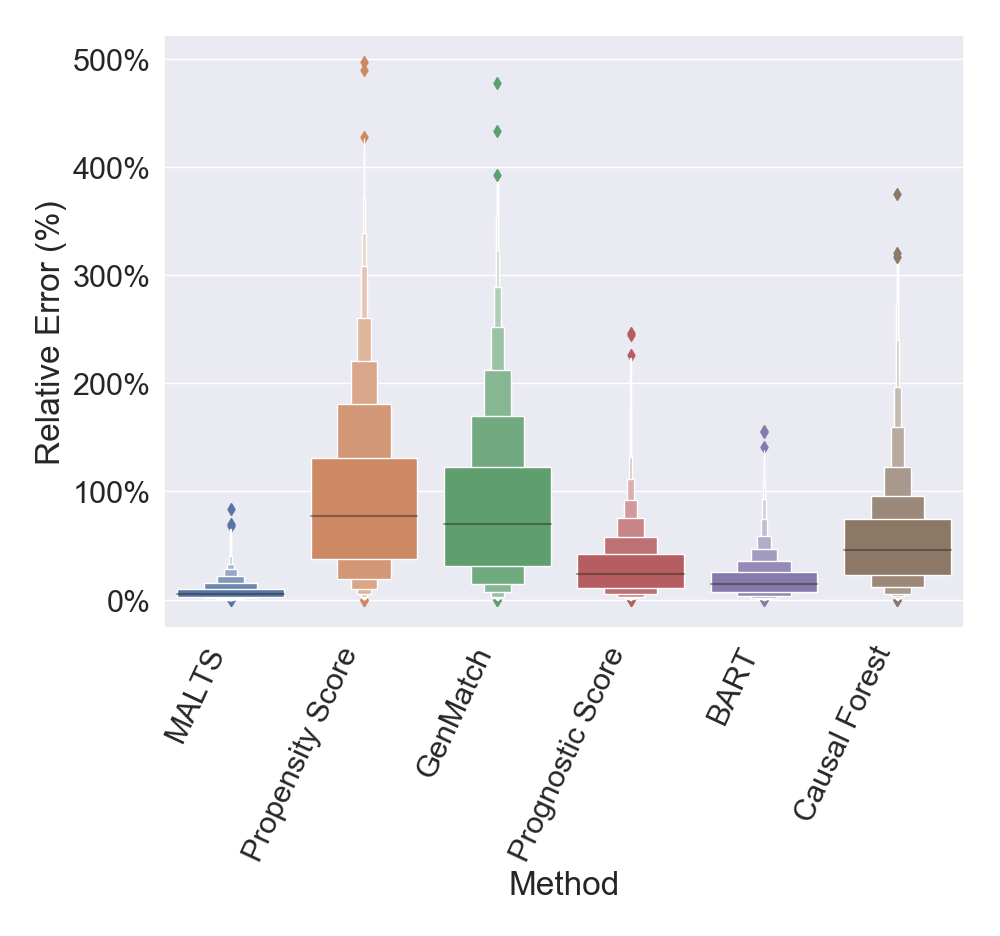
\includegraphics[width=0.7\textwidth]{Figures/boxplot_multifold_malts_continuous.png}    \caption{{\textit{\it MALTS performs well with respect to other methods for continuous data.}} Letter-box plots of CATE Absolute Error on the test set for several methods.}
    \label{fig:continuous}
\end{figure}


% \begin{figure}[h]
%     \centering
%     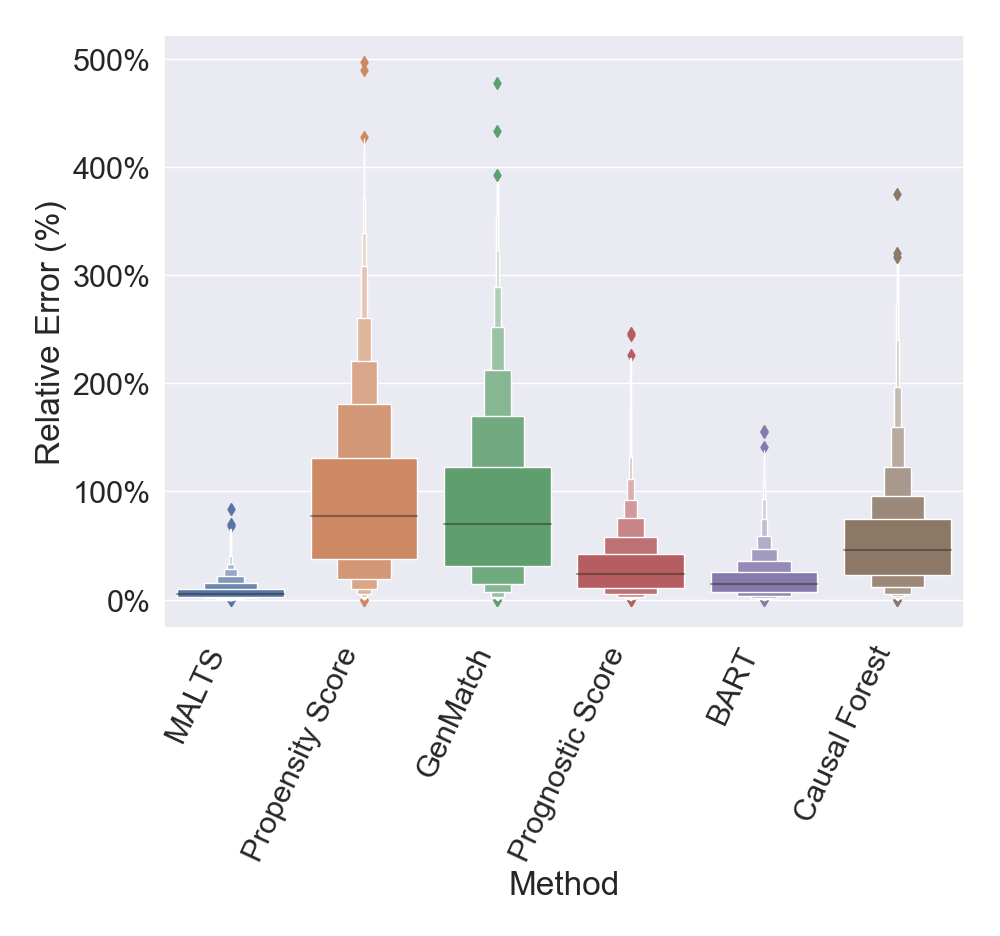
\includegraphics[width=0.85\textwidth]{Figures/boxplot_multifold_malts_continuous.png}\\
%     (a) Continuous Covariates\\
%     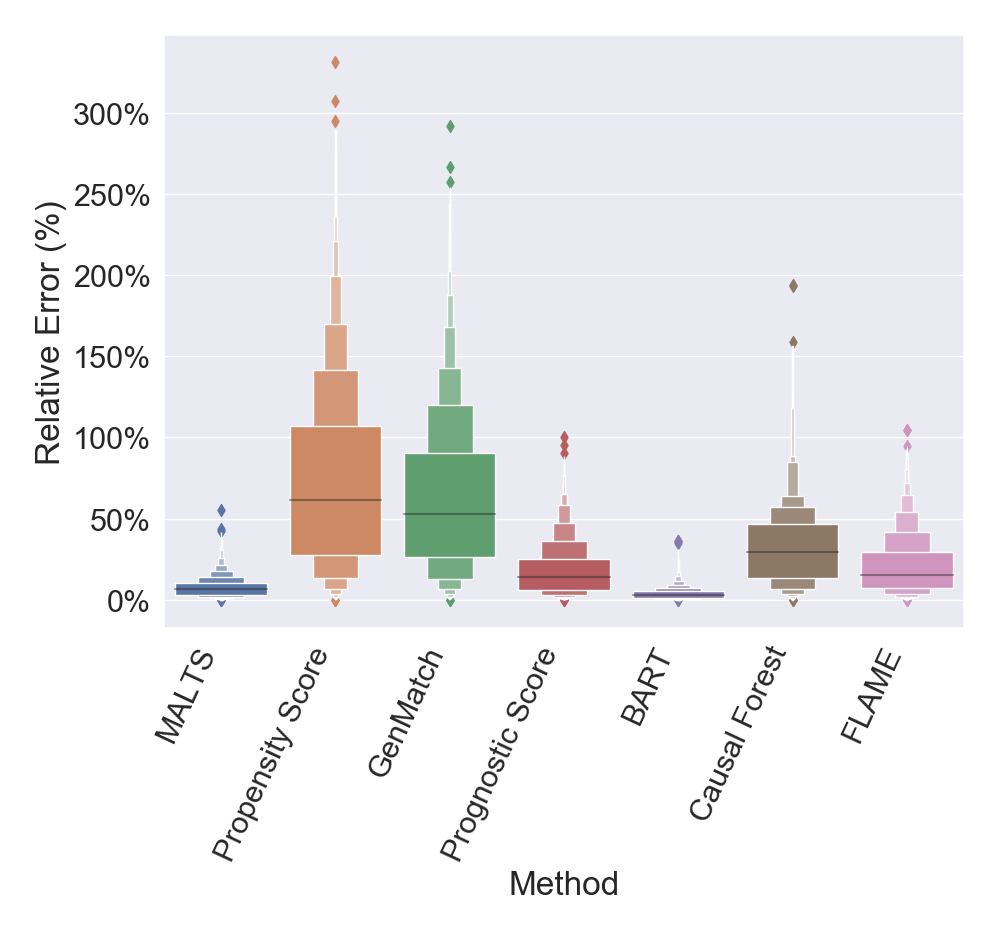
\includegraphics[width=0.9\textwidth]{Figures/boxplot_multifold_malts_discrete.png}\\
%     (b) Discrete Covariates
    
%     \caption{{\textit{\it MALTS performs well with respect to other methods.}} Letter-box plots of CATE Absolute Error on the test set for several methods. MALTS performs well, despite being a matching method, on the setup with (a) continuous covariates, (b) discrete covariates.}
%     \label{fig:continuous}
% \end{figure}

%Figure~\ref{fig:continuous}(a) shows the performance of various causal inference methods on the simulated data. MALTS performance is on par with existing state-of-the-art methods like BART. The error-rate for MALTS is significantly lower compared to prognostic score matching or causal forest.

\subsection{Discrete Covariates}
We use the data-generative process described in Section~\ref{dgp1} to generate 2500 units with no continuous covariates, 15 important discrete covariates and 10 irrelevant discrete covariates. Further, we set the parameters to the DGP as follows:
$\mu = 1$, $\Sigma = 1.5$, $\phi=0.5$, $\sigma = 20$ and $c = 2$. We used the weighted Hamming distance metric for this experiment.
%We compared the CATE estimation error-rates for MALTS in contrast with other existing matching and non-matching methods.

% \begin{figure}
%     \centering
%     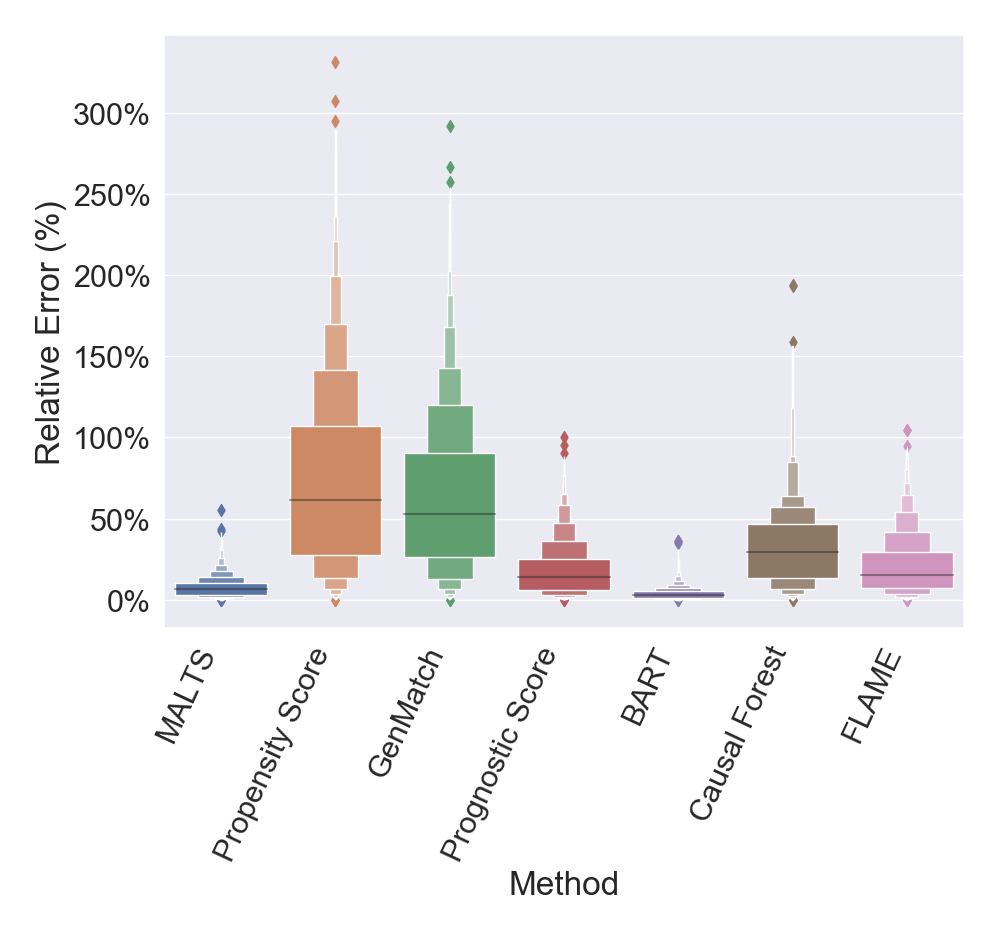
\includegraphics[width=0.9\textwidth]{Figures/boxplot_multifold_malts_discrete.png}
%     \caption{Discrete Covariates}
%     \label{fig:discrete}
% \end{figure}

Figure~\ref{fig:discrete} shows the performance comparison, again showing that 
%of various causal inference methods on the simulated data. 
MALTS' performance is on par with existing state-of-the-art non-matching methods; it also performs better than FLAME (a state-of-the-art matching method for discrete data) as it is able to provide additional smoothing in this relatively small-$n$ setting. \textit{Hence, MALTS performs well for discrete covariates in the quadratic data generation process.}
%methods like BART and the error-rate for MALTS is significantly lower compared to other treatment effect estimation methods prognostic score matching or FLAME.
\begin{figure}
     \centering
    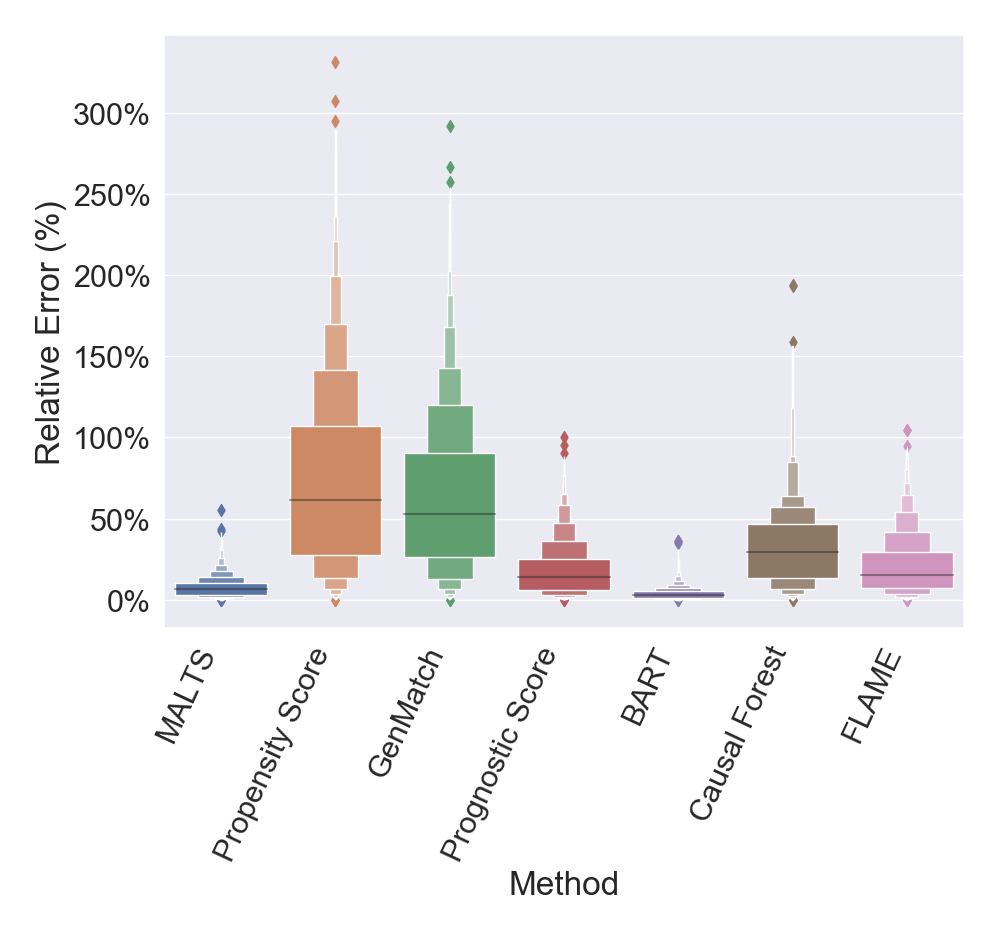
\includegraphics[width=0.65\textwidth]{Figures/boxplot_multifold_malts_discrete.png}    \caption{{\textit{\it MALTS performs well with respect to other methods for discrete data.}} Letter-box plots of CATE Absolute Error on the test set for several methods.}
    \label{fig:discrete}
\end{figure}


\subsection{Mixed Covariates}
We use the data-generative process used for experiments on continous and discrete covariates (described in Section~\ref{dgp1}) to generate 2500 units with 5 relevant continuous covariates, 15 relevant discrete covariates, 10 irrelevant continuous and 10 irrelevant discrete covariates. We used the same set of parameters for the DGP as the previous two experiments. Similarly to the previous two experiments, Figure~\ref{fig:mixed} shows that \textit{MALTS performs on par with the state-of-the-art non-matching methods and outperforms all matching methods that can handle mixed covariates for the quadratic data generation process.}

\begin{figure}[h]
    \centering
    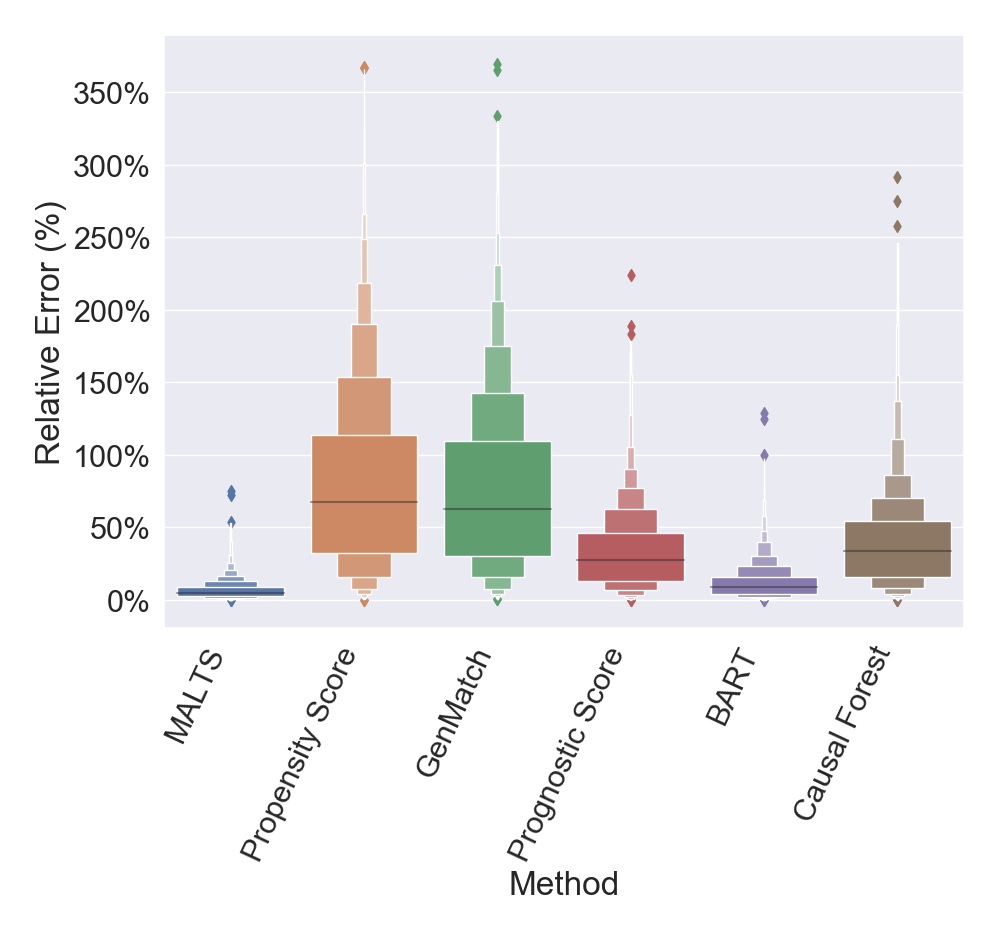
\includegraphics[width=0.65\textwidth]{Figures/boxplot_multifold_malts_mixed.png}
    \caption{{\textit{\it MALTS performs well on data with mixed covariates.}} Letter-box plots of CATE Absolute Error on the test set for several methods. MALTS performs well on the setup with mixed (continuous+discrete) covariates.}
    \label{fig:mixed}
\end{figure}

\subsection{Friedman's Setup}
We further compare MALTS and other flexible methods' performance on data generated using the process described in Section~\ref{dgp2}. 
%We test MALTS and other methods in the DGP mentioned in Section~\ref{dgp2} because the potential outcome functions for the 
This DGP is particularly interesting because the potential outcomes are highly non-linear functions with trigonometric expressions.

\begin{figure}[h]
    \centering
    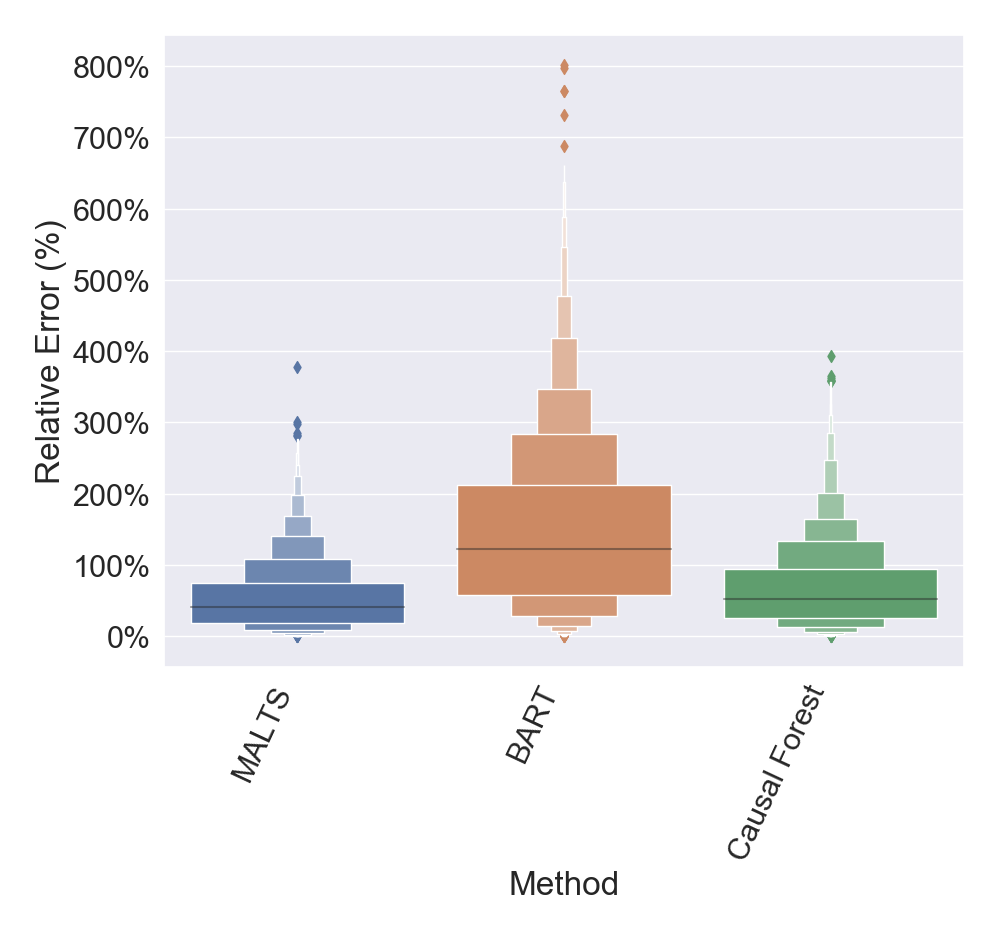
\includegraphics[width=0.65\textwidth]{Figures/boxplot_multifold_malts_friedman_2.png}
    \caption{{\textit{\it MALTS performs well on Friedman's setup.}} Letter-box plots of CATE Absolute Error on the test set for MALTS and two black box methods. 
    %MALTS performs well, despite being a matching method on Friedman's setup with highly non-linear setup with scale trigonometric treatment effect.
    }
    \label{fig:Friedman}
\end{figure}

As shown in Figure~\ref{fig:Friedman}, we observe that \textit{MALTS performs on par with Causal Forest while BART's error-rate is significantly higher (worse) than MALTS, for the Friedman's data generation process}. 

% Based on the experiments comparing the error-rates of various CATE estimation procedures across different simulation setups, MALTS (while being interpretable) also can perform on par or better than the existing methods. 

% We further analyzed MALTS' variance estimates and performance under limited overlap between the covariates' distribution of treated and control groups, shown in Appendix~B. 

%In next subsection, we use MALTS along with other causal inference methods to estimate treatment effect and compare their performance on Lalonde's temporary employment program data.

\subsection{LaLonde Data}
The LaLonde data pertain to the National Support Work Demonstration (NSW) temporary employment program and its effect on income level of the participants \citep{lalonde}. This dataset is frequently used as a benchmark for the performance of methods for observational causal inference. We employ the male sub-sample from the NSW in our analysis as well as the PSID-2 control sample of male household-heads under age 55 who did not classify themselves as retired in 1975 and who were not working when surveyed in the spring of 1976 \citep{dehejia_wahba_nonexp}. The outcome variable for both experimental and observational analyses is earnings in 1978 and the considered variables are age, education, whether a respondent is Black, is Hispanic, is married, has a degree, and their earnings in 1975. Previously, it has been demonstrated that almost any adjustment during the analysis of the experimental and observational variants of these data (both by modeling the outcome and by modeling the treatment variable) can lead to extreme bias in the estimate of average treatment effects \citep{lalonde}.

\begin{table}
 \caption{{\it Predicted ATE for different methods on Lalonde's NSW experimental dataset. The MALTS estimate of ATE is closer to the true ATE than other methods.}}
 \label{tab:lalonde}
 \centering
\begin{tabular}{lrr}
\hline
{} &  \textbf{ATE Estimate} &  \textbf{Estimation Bias (\%)} \\
\textbf{Method}           &               &                      \\
\hline
Truth         &    886 &            - \\
\textit{MALTS}            &    \textit{881.67} &            \textit{-0.49} \\
\textit{MALTS  (pruned)}            &    \textit{888.53} &            \textit{0.29} \\
GenMatch         &    859.72 &            -2.97 \\
Propensity Score &    513.30 &           -42.06 \\
Prognostic Score &    943.81 &             6.52 \\
BART-CV          &   1164.72 &            31.46 \\
Causal Forest-CV &    509.32 &           -42.51 \\
\hline
\end{tabular}
\end{table}

\begin{table}
 \caption{{\it Predicted ATE for different methods on Lalonde's NSW experimental data and PSID-2 observational dataset.} We provide estimates for MALTS before and after pruning the matched groups with large diameters. The threshold to prune was chosen by rule of thumb on diameters of matched groups as shown in Figure~\ref{fig:lalonde_prune}(b).}
 \label{tab:lalonde_psid2}
 \centering
\begin{tabular}{lrr}
\hline
{} &  \textbf{ATE Estimate} &  \textbf{Estimation Bias (\%)} \\
\textbf{Method}          &               &                      \\
\hline
Truth         &    886 &            - \\
\textit{MALTS}            &    \textit{608.37} &             \textit{-31.34} \\
\textit{MALTS (pruned)}            &    \textit{891.75} &             \textit{0.65} \\
GenMatch         &    549.53 &           -37.98 \\
Propensity Score &    513.79 &           -42.01 \\
Prognostic Score &   -897.76 &          -201.33 \\
BART-CV          &    713.20 &           -19.50 \\
Causal Forest-CV &   -179.98 &          -120.31 \\
\hline
\end{tabular}
\end{table}

\textbf{Performance results:} Tables~\ref{tab:lalonde} and \ref{tab:lalonde_psid2} present the average treatment effect estimates based on MALTS, state-of-the-art modeling methods, and matching methods. \textit{MALTS (after appropriately pruning low-quality matched groups) is able to achieve accurate ATE estimation on both experimental and observational datasets.}

Figure~\ref{fig:lalonde_prune} illustrates how the matched groups were pruned. There was a clear visual separation between high-quality matched groups, which had low diameters, and low-quality matched groups, with larger diameters.

%As illustrated in Figure~\ref{fig:lalonde_prune}, the thresholding criteria for the observational Lalonde dataset were determined using the visual observation on diameters of the matched group such that the clusters containing matched groups with large diameters is pruned. 

\begin{figure}
    \centering
    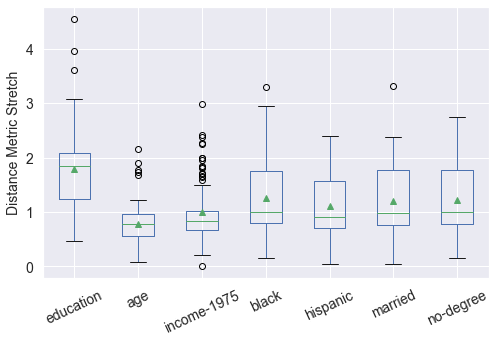
\includegraphics[width=0.75\textwidth]{Figures/m_lalonde.png}\\
    (a) Distance Metric learned on Lalonde data.\\
    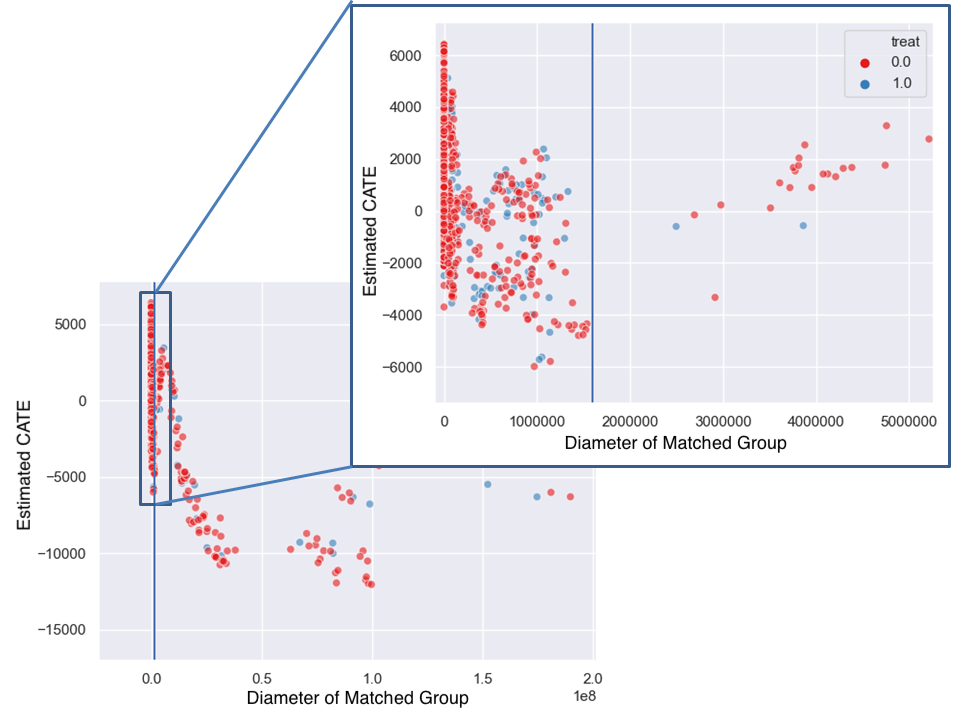
\includegraphics[width=0.9\textwidth]{Figures/lalonde_pruning.png}\\
    (b) Criteria for pruning low-quality matched groups.\\
    \caption{(a) Box-plot of distance metric stretch values corresponding to each covariate in Lalonde data learned over 100 estimations.  (b) Criteria to prune low-quality matched groups with large diameter from Lalonde data.}
    \label{fig:lalonde_prune}
\end{figure}

\textbf{Model Interpretability:}
One difference between MALTS and the other methods is that its solution can be described concisely: MALTS produces a total of seven numbers that define the distance metric. The distribution of the learned distance metric values across folds is shown in Figure~\ref{fig:lalonde_prune}(a). Once the researcher has these seven numbers, along with the value of $k$ in $k$-nearest neighbors used to train MALTS, they know precisely which units should be matched. In contrast, causal forest and BART require a model whose size  depends on the number of trees, where each tree is at least a couple of levels deep--in this case, 2000 trees  and 150 trees, respectively.

\textbf{Interpretability of Matched Groups:}
To examine the interpretability of MALTS' matched groups, we present two of the matched groups from MALTS for the observational Lalonde dataset in Table~\ref{tab:match-group-example}, corresponding to two ``query'' individuals in the dataset.
%We show the learned stretches for the distance metric ($\mathcal{M}$) in Figure~\ref{fig:lalonde_prune}(a). 
 %two individuals for whom we want to construct matched groups:
 Query 1 is a 22 year old with no income in 1975. We are able to construct a tight matched group for this individual (both in control and in treatment). In contrast, Query 2 is a 42-year-old high-income individual without a degree, which is an extremely unlikely scenario, leading to a matched group with a very large diameter, which should probably not be used during analysis. Such granular analysis is not possible for regression methods like BART and matching methods like progostic score or propensity score matching. Table~\ref{tab:mg_prog} in Appendix~D shows an example matched group using prognostic score matching for unit-id-1 (MALTS produces high-quality matched group for this unit as shown in Table~\ref{tab:match-group-example}).

 This further highlights the troubleshooting capabilities of interpretable matching methods: by identifying units that are poorly matched, we know exactly which units to study in more detail. In this case, it is possible that the ``degree'' field might have a data error, which means it would be better not to match this unit and to potentially follow up on the veracity of their responses.

\begin{table}[]
\caption{{\it Learned distance metric and examples of matched-groups on Lalonde Experimental treatment and Observational control datasets for two example query points drawn from the same datasets.} Query 1 represents a high quality (low diameter) matched group while Query 2 represents a poor quality (high diameter) matched group that could be discarded during analysis.}
\label{tab:match-group-example}
\resizebox{\textwidth}{!}{%
\begin{tabular}{rrrrrrrrrr}
\hline
\textbf{} &
  \textbf{} &
  \textbf{Age} &
  \textbf{Education} &
  \textbf{Black} &
  \textbf{Hispanic} &
  \textbf{Married} &
  \textbf{No-Degree} &
  \textbf{Income-1975} &
  \textbf{} \\ \hline
mean($Diag(\mathcal{M})$) & & 0.780 & 1.786 & 1.254 & 1.110 & 1.205 & 1.229 & 1.001 &  \\
std($Diag(\mathcal{M})$) & & 0.361 & 0.778 & 0.641 & 0.577 & 0.614 & 0.618 & 0.512 &  \\ \hline
\end{tabular}%
}
\vskip 5mm
\resizebox{\textwidth}{!}{%
\begin{tabular}{lrrrrrrrrr}
\hline
\textbf{Unit-id} &
  \textbf{Treated} &
  \textbf{Age} &
  \textbf{Education} &
  \textbf{Black} &
  \textbf{Hispanic} &
  \textbf{Married} &
  \textbf{No-Degree} &
  \textbf{Income-1975} &
  \textbf{Income-1978} \\ \hline
Query-1: \textit{1}   & 1.0 & 22.0 & 9.0  & 0.0 & 1.0 & 0.0 & 1.0 & 0.0 & 3595.89  \\  \hline
\textit{94}  & 1.0 & 23.0 & 8.0  & 0.0 & 1.0 & 0.0 & 1.0 & 0.0 & 3881.28  \\
\textit{330} & 0.0 & 22.0 & 8.0  & 0.0 & 1.0 & 0.0 & 1.0 & 0.0 & 9920.94  \\
\textit{299} & 0.0 & 22.0 & 9.0  & 1.0 & 0.0 & 0.0 & 1.0 & 0.0 & 0.00     \\
\textit{5}   & 1.0 & 22.0 & 9.0  & 1.0 & 0.0 & 0.0 & 1.0 & 0.0 & 4056.49  \\
\textit{82}  & 1.0 & 21.0 & 9.0  & 1.0 & 0.0 & 0.0 & 1.0 & 0.0 & 0.00     \\
\textit{416} & 0.0 & 22.0 & 9.0  & 1.0 & 0.0 & 0.0 & 1.0 & 0.0 & 12898.38 \\
\textit{333} & 0.0 & 21.0 & 9.0  & 1.0 & 0.0 & 0.0 & 1.0 & 0.0 & 3343.22  \\
\textit{292} & 1.0 & 20.0 & 9.0  & 1.0 & 0.0 & 0.0 & 1.0 & 0.0 & 8881.67  \\
\textit{17}  & 1.0 & 23.0 & 10.0 & 1.0 & 0.0 & 0.0 & 1.0 & 0.0 & 7693.40  \\
\textit{116} & 1.0 & 24.0 & 10.0 & 1.0 & 0.0 & 0.0 & 1.0 & 0.0 & 0.00     \\ \hline
\end{tabular}%
}
\vskip 5mm
\resizebox{\textwidth}{!}{%
\begin{tabular}{lrrrrrrrrr}
\hline
\textbf{Unit-id} &
  \textbf{Treated} &
  \textbf{Age} &
  \textbf{Education} &
  \textbf{Black} &
  \textbf{Hispanic} &
  \textbf{Married} &
  \textbf{No-Degree} &
  \textbf{Income-1975} &
  \textbf{Income-1978} \\
\hline
Query-2: \textit{968} &    0.0 &  42.0 &       11.0 &    0.0 &       0.0 &      1.0 &       1.0 &  44758.07 &  54675.88 \\
\hline
\textit{274} &    1.0 &  35.0 &        9.0 &    1.0 &       0.0 &      1.0 &       1.0 &  13830.64 &  12803.97 \\
\textit{141} &    1.0 &  25.0 &        8.0 &    1.0 &       0.0 &      0.0 &       1.0 &  37431.66 &   2346.83 \\
\textit{967} &    0.0 &  50.0 &       17.0 &    0.0 &       0.0 &      1.0 &       0.0 &  30435.48 &  25860.21 \\
\textit{948} &    0.0 &  35.0 &       12.0 &    0.0 &       0.0 &      1.0 &       0.0 &  26854.84 &  29554.53 \\
\textit{210} &    1.0 &  25.0 &        8.0 &    0.0 &       0.0 &      0.0 &       1.0 &  23096.65 &   6421.53 \\
\textit{241} &    1.0 &  24.0 &       15.0 &    1.0 &       0.0 &      0.0 &       0.0 &  13008.50 &  14683.63 \\
\textit{311} &    0.0 &  28.0 &       12.0 &    1.0 &       0.0 &      1.0 &       0.0 &  29009.11 &  10067.43 \\
\textit{183} &    1.0 &  23.0 &       10.0 &    1.0 &       0.0 &      0.0 &       1.0 &  15709.56 &   5665.07 \\
\textit{182} &    1.0 &  23.0 &       12.0 &    1.0 &       0.0 &      1.0 &       0.0 &  15079.95 &  10283.49 \\
\hline
\end{tabular}
%
}
\end{table}
	% !TEX root = main.tex
\section{Conclusion and Discussion}\label{sec:Conclusion}
This paper introduces the MALTS algorithm, which learns a distance-metric on the covariate space for use with matching. The learned metric stretches important covariates and compresses irrelevant covariates for outcome prediction in order to produce high-quality matches. 
%MALTS is able to deal with irrelevant covariates by downweighting their importance in the weighted nearest neighbor algorithm that produces the matches. 
Unlike black-box machine learning methods, MALTS produces interpretable matched groups and returns the stretch matrix on covariates for counterfactual prediction. The stretch matrix is chosen here to be diagonal, so that it can be represented using only a few ``stretch'' numbers that determine the importance of each covariate in determining the matched groups. The matched groups arising from these stretch matrices and are thus interpretable.

A natural extension that we are pursuing is to use neural networks or support vector machines to learn a flexible distance metric in a latent space, thus allowing us to match on medical records, images, and text documents.  This will allow us to incorporate complex data structures by introducing a flexible learning framework (e.g., neural networks) for coding the data. That is, we can redefine the distance metric via
\begin{eqnarray*}\nonumber
\textrm{distance}_{\mathcal{M}} (\x_i,\x_j) &=& \langle\phi_{\mathcal{M}}(\x_i),\phi_{\mathcal{M}}(\x_j) \rangle \;\;\;\textrm{or}\\\nonumber
\textrm{distance}_{\mathcal{M}} (\x_i,\x_j) &=& \left(\phi_{\mathcal{M}}(\x_i)-\phi_{\mathcal{M}}(\x_j)\right)^2,
\end{eqnarray*}
where $\phi$ is a summary of relevant data features learned using a complex modeling framework. As deep neural networks mainly show improvements over other methods for problems that do not have natural data representations (computer vision, speech, etc.), we conjecture that the stretch/almost-exact match combination should suffice for most datasets. The MALTS framework can be further extended to deal with missing covariates, and can be adapted to instrumental variables. 

	

	
	\acks{This work supported by DHHS, PHS, NIH, and NIBI under grant 1R01EB025021-01, and also by the Duke Energy Initiative.}

% 	\bibliographystyle{natbib}
 	\bibliography{biblio}{}
	
\appendix

    % !TEX root = main.tex
\section*{Appendix A}
In this section we provide proofs for theorems and lemmas discussed in Section~\ref{sec:theory}.\\\\
\allowdisplaybreaks
% \textbf{Proof (Theorem~\ref{th: robust})}. Given $\mathcal{Z}=\mathcal{X}\times\mathcal{Y}\times\mathcal{T}$, we consider the following definition of a minimum sized $\gamma$-cover $\hat{\mathcal{V}}$ of the set $\mathcal{X}$ under the distance metrix $\|\cdot\|_2$: Partition the set into $K$ disjoint subsets $\{C_i\}_{i=1}^{K}$ such that $K$ is the $\gamma$-covering-number of $\mathcal{X}$ under $\|\cdot\|_2$ (which is exactly equal to $|\hat{\mathcal{V}}|$) where each $C_i$ is the $\gamma$-neighborhood of each $\hat{v}_i\in\hat{\mathcal{V}}$ and each $C_i$ contains at least one control and one treated sample. Note that if such a cover exists, then since $\mathcal{X}$ is a compact convex set, $K$ is finite. 

% We further assume that distance metric $\|\cdot\|_2$ is a smooth distance metric with bounding function $\delta(\cdot)$. This implies that $\delta(\cdot)$ is a monotonically increasing zero-intercept function such that $\forall z_1,z_2 \in \mathcal{Z}$ if $t_1=t_2$ and $\|\x_1-\x_2\|_2\leq\epsilon$ then $|y_1-y_2|\leq\delta(\epsilon)$. This further implies that for any $z_1$ and $z_2$ such that $x_1, x_2 \in C_{i}$ and $t_1=t_2$ then, since they are both in the same ball of radius $\gamma$, we have $|y_1-y_2|\leq\delta(\gamma)$.

% For some $s_1=(\x_1,y_1,t_1)$ and $s_2=(\x_2,y_2,t_2)$ in the training set $\mathcal{S}_n$ and $z_1=(\x'_1,y'_1,t'_1)$ and $z_2=(\x'_2,y'_2,t'_2)$ in $\mathcal{Z}$ such that $\x_1,\x'_1\in C_{i}$, $\x_2,\x'_2\in C_{l}$, and $t_1=t'_1=t_2=t'_2$, then we try to bound the following quantity: $$\Big|loss[\mathcal{M}(\mathcal{S}_n),s_1,s_2]-loss[\mathcal{M}(\mathcal{S}_n),z_1,z_2]\Big| = \Big| |e^{-\dis_{\mathcal{M}(\mathcal{S}_n)}(\x_1,\x_2)} (y_1-y_2)| - |e^{-\dis_{\mathcal{M}(\mathcal{S}_n)}(\x'_1,\x'_2)} (y'_1 - y'_2)| \Big|.$$
% From the reverse triangle inequality we know
% \begin{eqnarray*}
%   \lefteqn{
%   \Big| |e^{-\dis_{\mathcal{M}(\mathcal{S}_n)}(\x_1,\x_2)} (y_1-y_2)| - |e^{-\dis_{\mathcal{M}(\mathcal{S}_n)}(\x'_1,\x'_2)} (y'_1 - y'_2)| \Big|
%   }\\
%   &\leq&
%   \Big| e^{-\dis_{\mathcal{M}(\mathcal{S}_n)}(\x_1,\x_2)} (y_1-y_2) - e^{-\dis_{\mathcal{M}(\mathcal{S}_n)}(\x'_1,\x'_2)} (y'_1 - y'_2) \Big|\\
%   &=&
%           \Big| e^{-\dis_{\mathcal{M}(\mathcal{S}_n)}(\x_1,\x_2)} y_1 - e^{-\dis_{\mathcal{M}(\mathcal{S}_n)}(\x_1,\x_2)} y_1 +   e^{-\dis_{\mathcal{M}(\mathcal{S}_n)}(\x'_1,\x'_2)} y_1 
%   - e^{-\dis_{\mathcal{M}(\mathcal{S}_n)}(\x'_1,\x'_2)} y'_1 
%   \\&&- e^{-\dis_{\mathcal{M}(\mathcal{S}_n)}(\x_1,\x_2)} y_2 + e^{-\dis_{\mathcal{M}(\mathcal{S}_n)}(\x'_1,\x'_2)} y_2 - e^{-\dis_{\mathcal{M}(\mathcal{S}_n)}(\x'_1,\x'_2)} y_2
%   + e^{-\dis_{\mathcal{M}(\mathcal{S}_n)}(\x'_1,\x'_2)} y'_2 \Big|\\
%   & =&
%   \Bigg| y_1 \Big( e^{-\dis_{\mathcal{M}(\mathcal{S}_n)}(\x_1,\x_2)}  - e^{-\dis_{\mathcal{M}(\mathcal{S}_n)}(\x'_1,\x'_2)} \Big) +   e^{-\dis_{\mathcal{M}(\mathcal{S}_n)}(\x'_1,\x'_2)} (y_1 - y'_1)
%   \\&&- y_2 \Big( e^{-\dis_{\mathcal{M}(\mathcal{S}_n)}(\x_1,\x_2)}  - e^{-\dis_{\mathcal{M}(\mathcal{S}_n)}(\x'_1,\x'_2)} \Big) - e^{-\dis_{\mathcal{M}(\mathcal{S}_n)}(\x'_1,\x'_2)} (y_2 - y'_2) \Bigg|,
% \end{eqnarray*}
% and applying the triangle inequality, 
% \begin{eqnarray*}
%   &\leq&
%   \Big| y_1 \Big( e^{-\dis_{\mathcal{M}(\mathcal{S}_n)}(\x_1,\x_2)}  - e^{-\dis_{\mathcal{M}(\mathcal{S}_n)}(\x'_1,\x'_2)} \Big)\Big| +  \Big| e^{-\dis_{\mathcal{M}(\mathcal{S}_n)}(\x'_1,\x'_2)} (y_1 - y'_1) \Big|
%   \\
%   &&+\Big| y_2 \Big( e^{-\dis_{\mathcal{M}(\mathcal{S}_n)}(\x_1,\x_2)} -  e^{-\dis_{\mathcal{M}(\mathcal{S}_n)}(\x'_1,\x'_2)} \Big) \Big| + \Big| e^{-\dis_{\mathcal{M}(\mathcal{S}_n)}(\x'_1,\x'_2)} (y_2 - y'_2) \Big|.
% \end{eqnarray*}
% For any $y\in \mathcal{Y}$, we know that $|y|\leq\mathbf{C}_y$. Thus,
% \begin{eqnarray*}
%   \lefteqn{
%   \Big| |e^{-\dis_{\mathcal{M}(\mathcal{S}_n)}(\x_1,\x_2)} (y_1-y_2)| - |e^{-\dis_{\mathcal{M}(\mathcal{S}_n)}(\x'_1,\x'_2)} (y'_1 - y'_2)| \Big|
%   }\\
%   &\leq&
%   2\mathbf{C}_y \Bigg( \Big| e^{-\dis_{\mathcal{M}(\mathcal{S}_n)}(\x_1,\x_2)}  - e^{-\dis_{\mathcal{M}(\mathcal{S}_n)}(\x'_1,\x'_2)}\Big|\Bigg) +  |y_1-y'_1| + |y_2-y'_2|.
% \end{eqnarray*}
% By the smoothness of distance metric $\|\cdot\|_2$ and the fact that the two points are in the same $\gamma$-sized ball, we know that $|y_1-y'_1| + |y_2-y'_2|\leq 2\delta(\gamma)$. Hence,
% \begin{eqnarray*}
% \lefteqn{\Big|loss[\mathcal{M}(\mathcal{S}_n),s_1,s_2]-loss[\mathcal{M}(\mathcal{S}_n),z_1,z_2]\Big|}\\
%   &\leq&
%   2\Bigg( \mathbf{C}_y \Big| e^{-\dis_{\mathcal{M}(\mathcal{S}_n)}(\x_1,\x_2)}  - e^{-\dis_{\mathcal{M}(\mathcal{S}_n)}(\x'_1,\x'_2)}\Big| +  \delta(\gamma) \Bigg).
% \end{eqnarray*}
% If we multiply the right-hand-side of the inequality with a number greater than 1, then the inequality will not change. Hence,
% \begin{eqnarray*}
%      \lefteqn{
%      2\Bigg(\mathbf{C}_y \Big| e^{-\dis_{\mathcal{M}(\mathcal{S}_n)}(\x_1,\x_2)} - e^{-\dis_{\mathcal{M}(\mathcal{S}_n)}(\x'_1,\x'_2)} \Big| + \delta(\gamma) \Bigg)}\\
%      &\leq&
%      2\Bigg(\mathbf{C}_y  \Big| e^{\dis_{\mathcal{M}(\mathcal{S}_n)}(z_1,z_2)-\dis_{\mathcal{M}(\mathcal{S}_n)}(\x_1,\x_2)} - 1 \Big| +  \delta(\gamma) \Bigg)\\
% %\end{equation}
% %\begin{equation}
%      &=&
%      2\Bigg(\mathbf{C}_y \Big| e^{(\x'_1-\x'_2)^T\mathcal{M}(\mathcal{S}_n)(\x'_1-\x'_2)-(\x_1-\x_2)^T\mathcal{M}(\mathcal{S}_n)(\x_1-\x_2)} - 1 \Big| + \delta(\gamma) \Bigg)\\
%      &=&
%      2\Bigg(\mathbf{C}_y \Big| exp\Bigg((\x'_1-\x'_2)^T\mathcal{M}(\mathcal{S}_n)(\x'_1-\x'_2) - (\x_1-\x_2)^T\mathcal{M}(\mathcal{S}_n)(\x'_1-\x'_2)
%      \\&&+ (\x_1-\x_2)^T\mathcal{M}(\mathcal{S}_n)(\x'_1-\x'_2) -(\x_1-\x_2)^T\mathcal{M}(\mathcal{S}_n)(\x_1-\x_2)\Bigg) - 1 \Big| + \delta(\gamma) \Bigg) \Bigg)\\
%      &=&
%      2\Bigg(\mathbf{C}_y \Big| exp\Bigg((\x'_1-\x'_2)^T\mathcal{M}(\mathcal{S}_n)(\x'_1 - \x'_2 - \x_1 + \x_2)
%      \\&&+ (\x_1-\x_2)^T\mathcal{M}(\mathcal{S}_n)(\x'_1 - \x'_2 - \x_1 + \x_2)\Bigg) - 1 \Big| + \delta(\gamma) \Bigg) \Bigg)\\
%      &=&
%      2\Bigg(\mathbf{C}_y \Big| exp\Bigg((\x'_1-\x'_2)^T\mathcal{M}(\mathcal{S}_n)(\x'_1 - \x_1) + (\x'_1-\x'_2)^T\mathcal{M}(\mathcal{S}_n)(\x_2 - \x'_2)
%      \\&&+ (\x_1-\x_2)^T\mathcal{M}(\mathcal{S}_n)(\x'_1 - \x_1) + (\x_1-\x_2)^T\mathcal{M}(\mathcal{S}_n)(\x_2 - \x'_2)\Bigg) - 1 \Big| + \delta(\gamma) \Bigg) \Bigg)\\
%      &\leq& 
%      2\Bigg( \mathbf{C}_y \Bigg| \exp\Big( \|\x_1-\x_2\|_2\|\mathcal{M}(\mathcal{S}_n)\|_\mathcal{F}\|\x_1-\x'_1\|_2 
%      + \|\x_1-\x_2\|_2\|\mathcal{M}(\mathcal{S}_n)\|_\mathcal{F}\|\x_2-\x'_2\|_2 
%      \\&&+ \|\x'_1-\x'_2\|_2\|\mathcal{M}(\mathcal{S}_n)\|_\mathcal{F}\|\x_1-\x'_1\|_2
%      + \|\x'_1-\x'_2\|_2\|\mathcal{M}(\mathcal{S}_n)\|_\mathcal{F}\|\x_2-\x'_2\|_2 
%      \Big)
%       - 1 \Bigg| +  \delta(\gamma) \Bigg)\\
% %\end{split}
% %\end{equation}
% %\begin{equation}
%     &\leq& 2 \Bigg( \mathbf{C}_y  \Big| e^{4 \mathbf{C}_x \gamma \|\mathcal{M}(\mathcal{S}_n)\|_\mathcal{F} } - 1 \Big| + \delta(\gamma) \Bigg)
%     = 
%     2\mathbf{C}_y \Bigg( \Big| e^{4 \mathbf{C}_x \gamma g_0/c } - 1 \Big| \Bigg) +  2\delta(\gamma).
% \end{eqnarray*}
% Hence, we conclude that our fixed $\gamma$, the distance metric learned using \textsc{MALTS} algorithm is robust by the definition of robustness.

%---------------------------------------------

% proof for lemma 1

\textbf{Proof (Lemma~\ref{lm: whpavgloss})}. If $(D_1,\dots,D_K)$ is the multinomially distributed random vector with parameters $d$ and $p_1, \dots, p_K$ then, by the Bretagnolle-Huber-Carol inequality, $ P(\sum_{i=1}^{K} \Big| \frac{D_i}{d} - p_i \Big|\geq\lambda)\leq 2^K e^{-\frac{d\lambda^2}{2}}$. Thus, for our case, we can consider $N_i$ corresponding to the set of indices of units in sample $\mathcal{S}^{(t')}_n$ such that their $x$'s are contained in the partition $\mathbf{C}_{i}$ as in Theorem~\ref{th: robust}. Hence, by the Bretagnolle-Huber-Carol inequality, we know that 
$$
    P\Bigg(~ \sum_{i=1}^{K} \Big| \frac{|N_i|}{n^{(t')}} - \mu(\mathbf{C}_{i}) \Big| \geq \sqrt{\frac{2K~\ln(2)~+~2~\ln(1/\mathcal{E})}{n^{(t')}}} ~\Bigg) \leq \mathcal{E}~.
$$
Now, for some arbitrary $t'\in\mathcal{T}$ let us consider $\Big| L_{pop}(\mathcal{M}(\mathcal{S}_n),\mathcal{Z}^{(t')}) - L_{emp}(\mathcal{M}(\mathcal{S}_n),\mathcal{S}_n^{(t')}) \Big|$. 
We know that
{\allowdisplaybreaks
\begin{eqnarray*}
%   \begin{split}
\lefteqn{
        \Big| L_{pop}(\mathcal{M}(\mathcal{S}_n),\mathcal{Z}^{(t')}) - L_{emp}(\mathcal{M}(\mathcal{S}_n),\mathcal{S}_n^{(t')}) \Big| }\\
       & =& 
        \Bigg| \sum_{i,j=1}^{K} \Big( \mathbb{E}_{z_1,z_2}[loss(\mathcal{M}(\mathcal{S}_n),z_1=(\x'_1,y'_1,t'_1),z_2=(\x'_2,y'_2,t'_2))~|~\x'_1\in\mathbf{C}_i,\x'_2\in\mathbf{C}_j]~\mu(\mathbf{C}_i)\mu(\mathbf{C}_j) \Big)
        \\&&- 
        \frac{1}{(n^{(t')})^2}\sum_{s_1,s_2\in\mathcal{S}^{(t')}_n} loss(\mathcal{M}(\mathcal{S}_n),s_1,s_2)
        \Bigg|\\
        & =& 
        \Bigg| \sum_{i,j=1}^{K} \left( \mathbb{E}_{z_1,z_2}[loss(\mathcal{M}(\mathcal{S}_n),z_1,z_2)~|~\x'_1\in\mathbf{C}_i,\x'_2\in\mathbf{C}_j]~\mu(\mathbf{C}_i)\mu(\mathbf{C}_j) \right) \\&& - \sum_{i,j=1}^{K} \left(\mathbb{E}_{z_1,z_2}[loss(\mathcal{M}(\mathcal{S}_n),z_1,z_2)~|~\x'_1\in\mathbf{C}_i,\x'_2\in\mathbf{C}_j]~\mu(\mathbf{C}_i)~\frac{|N_j|}{n^{(t')}}\right)
        \\&&
        + \sum_{i,j=1}^{K} \left(\mathbb{E}_{z_1,z_2}[loss(\mathcal{M}(\mathcal{S}_n),z_1,z_2)~|~\x'_1\in\mathbf{C}_i,\x'_2\in\mathbf{C}_j]~\mu(\mathbf{C}_i)~\frac{|N_j|}{n^{(t')}}\right) \\&&+ \sum_{i,j=1}^{K} \mathbb{E}_{z_1,z_2}[loss(\mathcal{M}(\mathcal{S}_n),z_1,z_2)~|~\x'_1\in\mathbf{C}_i,\x'_2\in\mathbf{C}_j]~
        \frac{|N_i|}{n^{(t')}} \frac{|N_j|}{n^{(t')}} \\&&- \sum_{i,j=1}^{K} \mathbb{E}_{\x'_1,\x'_2}[loss(\mathcal{M}(\mathcal{S}_n),z_1,z_2)~|~\x'_1\in\mathbf{C}_i,\x'_2\in\mathbf{C}_j]~
        \frac{|N_i|}{n^{(t')}} \frac{|N_j|}{n^{(t')}}
        \\&&- 
        \frac{1}{(n^{(t')})^2}\sum_{s_1,s_2\in\mathcal{S}^{(t')}_n} loss(\mathcal{M}(\mathcal{S}_n),s_1,s_2)
        \Bigg|\\
        &\leq& \Bigg| \sum_{i,j=1}^{K} \mathbb{E}_{z_1,z_2}[loss(\mathcal{M}(\mathcal{S}_n),z_1,z_2)~|~\x'_1\in\mathbf{C}_i,\x'_2\in\mathbf{C}_j]~\mu(\mathbf{C}_i)\Big(\mu(\mathbf{C}_j) - \frac{|N_j|}{n^{(t')}}\Big) \Bigg|\\
        &&+\Bigg| \sum_{i,j=1}^{K} \mathbb{E}_{z_1,z_2}[loss(\mathcal{M}(\mathcal{S}_n),z_1,z_2)~|~\x'_1\in\mathbf{C}_i,\x'_2\in\mathbf{C}_j]~
        \frac{|N_j|}{n^{(t')}}
        \Big(\mu(\mathbf{C}_i) - \frac{|N_i|}{n^{(t')}}\Big) \Bigg|\\
       && + \Bigg| \sum_{i,j=1}^{K} \mathbb{E}_{z_1,z_2}[loss(\mathcal{M}(\mathcal{S}_n),z_1,z_2)~|~\x'_1\in\mathbf{C}_i,\x'_2\in\mathbf{C}_j]~
        \frac{|N_i|}{n^{(t')}} \frac{|N_j|}{n^{(t')}} \\&& - \frac{1}{(n^{(t')})^2}\sum_{s_1,s_2\in\mathcal{S}^{(t')}_n} loss(\mathcal{M}(\mathcal{S}_n),s_1,s_2) \Bigg|\\
    &\leq& 2B\sum_{i=1}^{K}\Big| \frac{|N_i|}{n^{(t')}} - \mu(\mathbf{C}_i) \Big| + \Bigg| \sum_{i,j=1}^{K} \mathbb{E}_{z_1,z_2}[loss(\mathcal{M}(\mathcal{S}_n),z_1,z_2)~|~\x'_1\in\mathbf{C}_i,\x'_2\in\mathbf{C}_j]~
        \frac{|N_i|}{n^{(t')}} \frac{|N_j|}{n^{(t')}} \\&& - \frac{1}{(n^{(t')})^2}\sum_{s_1,s_2\in\mathcal{S}^{(t')}_n} loss(\mathcal{M}(\mathcal{S}_n),s_1,s_2) \Bigg| \text{ where $B$ is }\max_{z_1,z_2} loss(\mathcal{M}(\mathcal{S}_n),z_1,z_2).
\end{eqnarray*}
}
Hence, we can conclude for all $t'\in\mathcal{T}$ we have
\begin{eqnarray*}
   & P_{\mathcal{S}_n}\Bigg( \Big| L_{pop}(\mathcal{M}(\mathcal{S}_n),\mathcal{Z}^{(t')}) - L_{emp}(\mathcal{M}(\mathcal{S}_n),\mathcal{S}_n^{(t')}) \Big| \geq \epsilon(\mathcal{S}^{(t')}_n) + 2B\sqrt{\frac{2K~\ln(2)~+~2~\ln(1/\mathcal{E})}{n^{(t')}}} \Bigg) \\
    &\leq 1 - (1-\mathcal{E})(p_{mr}(\epsilon))^{K^2}~.
\end{eqnarray*}
For notational simplicity, we do not consider ties here, though in our code, ties are handled by random selection.

%-------------------------------------------------

\begin{lemma}
\label{lm: smoothy}
Given a smooth distance metric $\mathcal{M}$ and treatment choice variable $t'\in\mathcal{T}$, if we estimate the counterfactual $\hat{y}^{(t')}(\x)$ for any given $z = (\x,y,t) \in \mathcal{Z}$  by nearest neighbor matching on a finite sample $\mathcal{S}_n \overset{i.i.d}{\sim}\mu(\mathcal{Z}^n)$ using distance metric $\mathcal{M}$, then the estimated counterfactual $\hat{y}^{(t')}(\x)$ and the true counterfactual $y^{(t')}(\x)$ are farther than $\epsilon$ with probability less than $\delta(\epsilon,\mathcal{M},n)$,
$$ P_{\mathcal{S}_n \sim \mu(\mathcal{Z}^n)}\Big( |\hat{y}^{(t')}(\x) - y^{(t')}(\x)| \geq \epsilon \Big) \leq \delta(\epsilon,\mathcal{M},n). $$
\end{lemma}

%-------------------------------------------------

\textbf{Proof (Lemma~\ref{lm: smoothy})}.
Let $\mathcal{B}_{\mathcal{M}}(\x,r)$ be an open ball of radius $r>0$ under distance metric $\mathcal{M}$, centered around point a fixed point $\x \in \mathcal{X}$. We know that there is a nonzero probability mass around any point $\x \in \mathcal{X}$,  
\begin{equation}
    \forall r>0, P_{X \sim \mu(\mathcal{X})}(X \in \mathcal{B}_{\mathcal{M}}(\x,r))>0.
\end{equation}

As $\mathcal{S}_n = \{Z_1=(X_1,Y_1,T_1),
\dots, Z_n=(X_n,Y_n,T_n)\} \overset{i.i.d}{\sim}\mu(\mathcal{Z})$, the probability that no unit $Z_i$ with $T_i=t'$ from a $n$-sized random sample $\mathcal{S}_n=\{Z_i\}^n_{i=1}$ lies within the $r$-neighborhood of a given unit $z=(\x,y,t) \in \mathcal{Z}$ is
\begin{equation}
    \label{eq: notinball}
    P_{\mathcal{S}_n \sim \mu(\mathcal{Z}^n) }\Bigg(
    \bigwedge_{Z_i\in\mathcal{S}_n} \Big(X_i \notin \mathcal{B}_{\mathcal{M}}(\x,r) \land T_i = t'\Big) \Bigg)
    \leq 
     P_{\mathcal{S}_n \sim \mu(\mathcal{Z}^n) }\Bigg(
    \bigwedge_{Z_i\in\mathcal{S}_n} \Big(X_i \notin \mathcal{B}_{\mathcal{M}}(\x,r) \Big) \Bigg)
    % =
    % \Big(1 - P_{X\sim\mu(\mathcal{X})}(X \in \mathcal{B}_{\mathcal{M}}(x,r))\Big)^{n} .
\end{equation}

\begin{equation}
    P_{\mathcal{S}_n \sim \mu(\mathcal{Z}^n) }\Bigg(
    \bigwedge_{Z_i\in\mathcal{S}_n} \Big(X_i \notin \mathcal{B}_{\mathcal{M}}(\x,r) \Big) \Bigg)
    =
    \Big(1 - P_{X\sim\mu(\mathcal{X})}(X \in \mathcal{B}_{\mathcal{M}}(\x,r))\Big)^{n} .
\end{equation}

From Equation~\ref{eq: notinball}, we can deduce that the probability that every unit with $T_i=t'$ in randomly drawn sample $\mathcal{S}_n$ is at least at a distance $r$ from a given $z=(\x,y,t)$ is 
\begin{equation}
\label{eq: notnearr}
    P_{\mathcal{S}_n \sim \mu(\mathcal{Z}^n)}\Big(\min_{\substack{Z_i\in\mathcal{S}_n\\T_i=t'}} \dis_{\mathcal{M}}(X_i,\x) \geq r \Big) 
    \leq
    \Big(1 - P_{X\sim\mu(\mathcal{X})}(X \in \mathcal{B}_{\mathcal{M}}(\x,r))\Big)^{n}.
\end{equation}
We infer from Equation~\ref{eq: notnearr} that
\begin{equation}
\label{eq: notnearrnn}
    P_{\mathcal{S}_n \sim \mu(\mathcal{Z}^n)}\Big(\dis_{\mathcal{M}}(1NN^{\mathcal{S}_n}_{\mathcal{M}}(\x,t'),\x) \geq r \Big) 
    \leq 
    \Big(1 - P_{X\sim\mu(\mathcal{X})}(X \in \mathcal{B}_{\mathcal{M}}(\x,r))\Big)^{n}.
\end{equation}

Combining the smoothness of distance metric $\dis_\mathcal{M}$, the counterfactual estimation $\hat{y}^{(t')}(\x)$ = $y\Big(1NN^{\mathcal{S}_n}_{\mathcal{M}}(\x,t')\Big)$ and Equation~\ref{eq: notnearrnn}, we infer that for some $\epsilon_r$ corresponding any $r>0$ we have:
\begin{eqnarray*}
    P_{\mathcal{S}_n \sim \mu(\mathcal{Z}^n)}\Big( |\hat{y}^{(t')}(\x) - y^{(t')}(\x)| \leq \epsilon_r \Big) \geq 
    \left(1-\beta_{\dis_\mathcal{M}}\right)\left(1-\Big(1 - P_{X\sim\mu(\mathcal{X})}(X \in \mathcal{B}_{\mathcal{M}}(\x,r))\Big)^{n}\right).
\end{eqnarray*}
\begin{eqnarray*}
    P_{\mathcal{S}_n \sim \mu(\mathcal{Z}^n)}\Big( |\hat{y}^{(t')}(\x) - y^{(t')}(\x)| \geq \epsilon_r \Big) \leq 1 -
    \left(1-\beta_{\dis_\mathcal{M}}\right)\left(1-\Big(1 - P_{X\sim\mu(\mathcal{X})}(X \in \mathcal{B}_{\mathcal{M}}(\x,r))\Big)^{n}\right).
\end{eqnarray*}
Hence, for any arbitrary $\epsilon$ we can always find a $\delta(\epsilon,\mathcal{M},n)$ such that 
\begin{equation}
  P_{\mathcal{S}_n \sim \mu(\mathcal{Z}^n)}\Big( |\hat{y}^{(t')}(\x) - y^{(t')}(\x)| \geq \epsilon \Big) \leq \delta(\epsilon,\mathcal{M},n). 
\end{equation}


Note that from Equation~\ref{eq: notnearrnn}, we can observe that $\lim_{n\to\infty}$ $1NN^{\mathcal{S}_n}_{\mathcal{M}}(\x,t) \to \x$; this implies \textit{asymptotic convergence of nearest neighbor}. We can also do a similar analysis for $KNN$ for any finite and fixed $K>0$, however for the sake of simplicity we have shown the finite sample bounds for $1NN$. In contract to previous works on nearest neighbor methods, the result shown Lemma~\ref{lm: smoothy} holds for any smooth distance metric, not just for a predefined distance metric.

%-------------------------------------------------

\begin{lemma}
\label{lm: ytotau}
If we can estimate the counterfactual %$\hat{y}^{(t)}(\cdot)$ 
using a finite sample $\mathcal{S}_n\overset{i.i.d}{\sim}\mu(\mathcal{Z}^n)$ such that the true counterfactual $y^{(t)}$ and the estimated counterfactual $\hat{y}^{(t)}(\cdot)$ are farther than $\epsilon'$ with probability less than $\delta'(\epsilon',\cdot,n)$ for any given $z\in\mathcal{Z}$ and $t \in \mathcal{T}$,
then the estimated individualized treatment $\hat{\tau}(\cdot)$ using a finite sample $\mathcal{S}_n\overset{i.i.d}{\sim}\mu(\mathcal{Z}^n)$ and the true individualized treatment effect $\tau(\cdot)$ are farther than $\epsilon$ with probability less than $\delta'(\frac{\epsilon}{2},\cdot,n)$.
$$ \forall t\in \mathcal{T}, ~P_{\mathcal{S}_n \sim \mu(\mathcal{Z}^n)}\Big( |\hat{y}^{(t)}(\x) - y^{(t)}(\x)| \geq \epsilon' \Big) \leq \delta'(\epsilon',\cdot,n) \implies P_{\mathcal{S}_n \sim \mu(\mathcal{Z}^n)}\Big( |\hat{\tau}(\x) - \tau(\x)| \geq \epsilon \Big) \leq \delta'\Big(\frac{\epsilon}{2},\cdot,n\Big). $$
\end{lemma}
\textbf{Proof (Lemma~\ref{lm: ytotau})}.
Given that for any $\epsilon'>$, we can find an $ \delta^{'}(\epsilon',\cdot,n)$ such that 
\begin{equation*}
    \forall z\in\mathcal{Z},~\forall t'\in \mathcal{T},~P_{\mathcal{S}_n \sim \mu(\mathcal{Z}^n)}(|\hat{y}^{(t')}(\x) - y^{(t')}(\x)|\geq \epsilon^{'})\leq \delta^{'}_{\epsilon^{'}}(\epsilon',\cdot,n).
\end{equation*}
We can further deduce that
\begin{equation}
    \label{eq: andeq}
    P\Bigg( \bigvee_{t'\in\mathcal{T}}~\Big(|\hat{y}^{(t')}(\x) - y^{(t')}(\x)| \geq \epsilon^{'}\Big) \Bigg) \leq |\mathcal{T}|~\delta^{'}(\epsilon',\cdot,n).
\end{equation}
By the triangle inequality, we also know that
\begin{equation}
\label{eq: treq1}
  \sum_{t'\in\mathcal{T}}\Big|\hat{y}^{(t')}(\x) - y^{(t')}(\x)\Big|
    \geq \Bigg| \sum_{t'\in\mathcal{T}}\Big(\hat{y}^{(t')}(\x) - y^{(t')}(\x)\Big) \Bigg|.
\end{equation}
Deducting from Equation~\ref{eq: andeq}, we have
\begin{equation*}
    P\Bigg( \sum_{t'\in\mathcal{T}}~\Big(|\hat{y}^{(t')}(\x) - y^{(t')}(\x)|\Big)  \geq |\mathcal{T}|\epsilon^{'}\Bigg) \leq |\mathcal{T}|~\delta^{'}(\epsilon',\cdot,n).
\end{equation*}
Applying the triangle inequality from Equation~\ref{eq: treq1},
\begin{equation*}
    P\Bigg( \Big| \sum_{t'\in\mathcal{T}}~\Big(\hat{y}^{(t')}(\x) - y^{(t')}(\x)\Big)\Big|  \geq |\mathcal{T}|\epsilon^{'}\Bigg) \leq |\mathcal{T}|~\delta^{'}(\epsilon',\cdot,n).
\end{equation*}
Considering the case where $\mathcal{T}=\{0,1\}$
\begin{equation*}
    P\Bigg( \Big| \hat{\tau}(\x) - \tau(\x)\Big|  \geq 2\epsilon^{'}\Bigg) \leq 2\delta^{'}(\epsilon',\cdot,n).
\end{equation*}
Hence, we can conclude that
\begin{equation*}
    P\Bigg( \Big| \hat{\tau}(\x) - \tau(\x)\Big|  \geq \epsilon\Bigg) \leq 2\delta^{'}\Big(\frac{\epsilon}{2},\cdot,n\Big).
\end{equation*}




    \section*{Appendix B}
\label{sec:var_overlap}
We use the DGP described in Section~\ref{dgp1} with 2 relevant continuous covariates and no irrelevant covariates for both the coverage and the limited overlap experiments. Further, we set the parameters to the DGP as follows:
$\mu = 1$, $\Sigma = 1.5$, $\phi=0.5$, $\sigma = 20$ and $c = 2$.
\subsection*{Coverage Study}
% WRITE ABOUT VARIANCE ESTIMATION PROCEDURE (MAYBE USE SOME OF THE TEXT FROM RESULTS SECTION).
We selected 9 reference points in a grid from the covariate space as shown in Figure~\ref{fig:Coverage}(b) and conducted an experiment that considered these reference points, over 100 repetitions. We compared coverage for CATEs estimated using MALTS for different values of variance, ranging from 1.0 to 4.0, for noise term $\epsilon_0$ and $\epsilon_1$ in the potential outcomes function. 

Variance estimation is notoriously hard in matching problems, even for overall quantities such as the average treatment effect \citep{doi:10.1111/j.1468-0262.2006.00655.x} and is part of ongoing work for the authors. We consider both the conservative variance estimator \citep{wang2017flame} and estimators that sacrifice some interpretability for better coverage. We consider the CATEs estimated using MALTS and study how well an uninterpretable method can predict those estimates. We use the predictive variance from gradient boosting regressor, from Gaussian Process regression and from Bayesian Ridge regression on the covariates and estimated average CATEs to quantify variance of each CATE estimate.

\begin{figure}
    \centering
    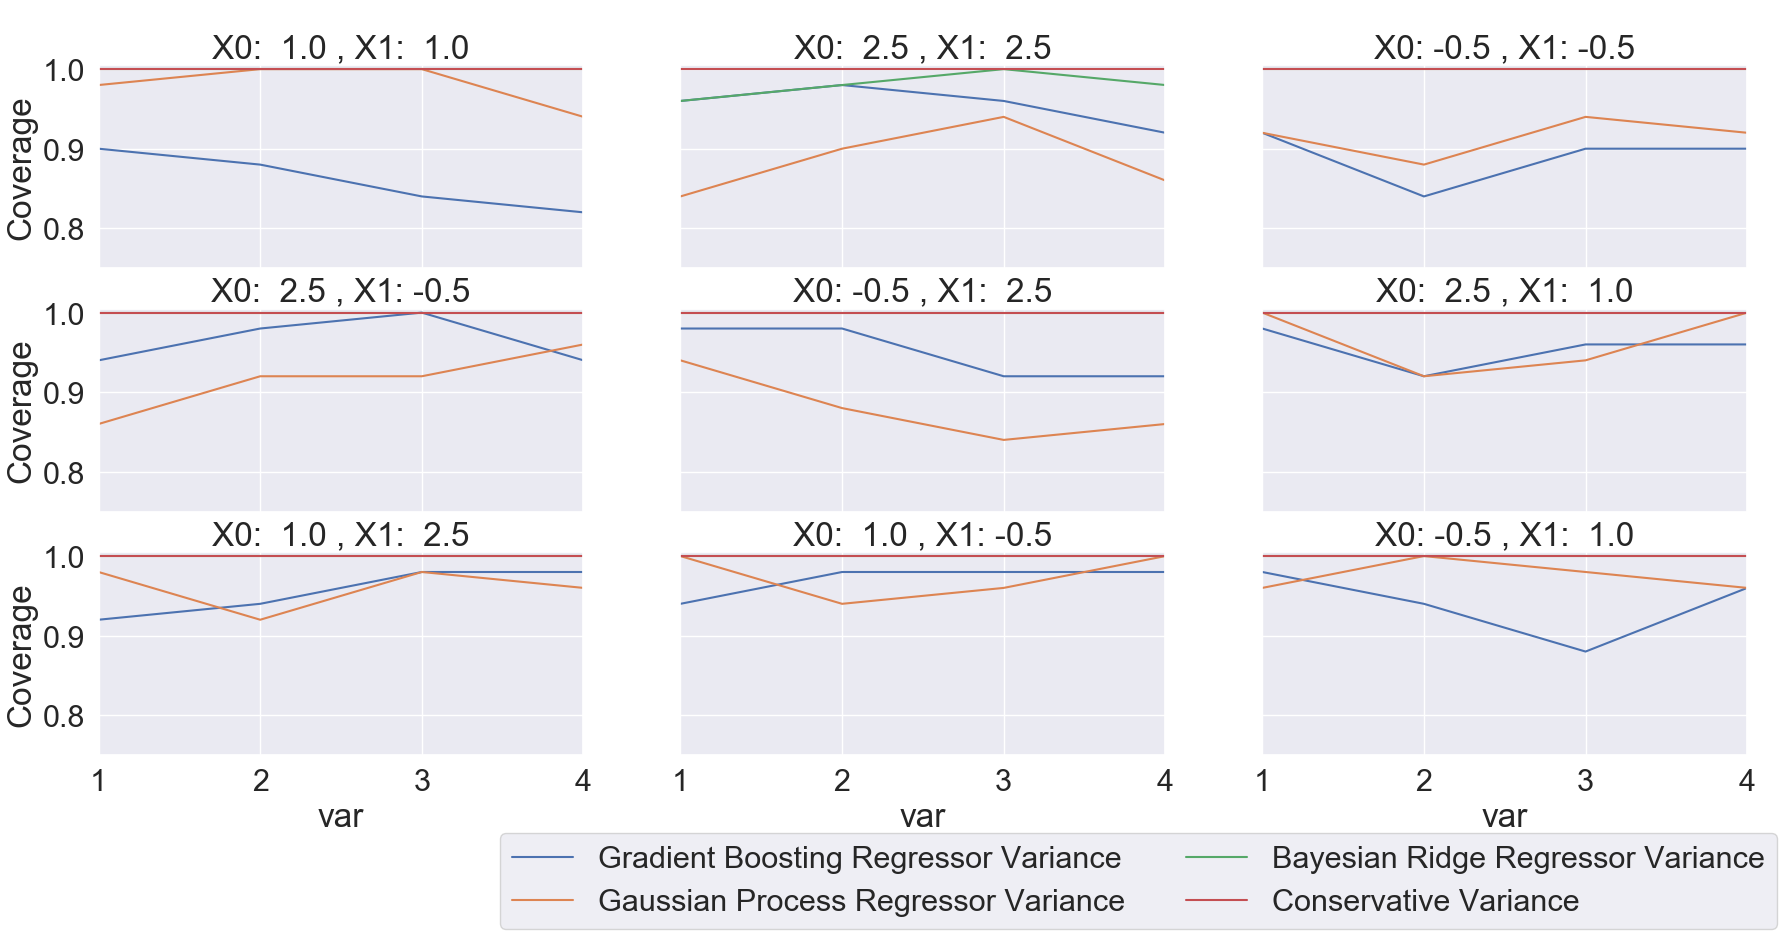
\includegraphics[width=\textwidth]{Figures/coverage.png}\\(a)\\
    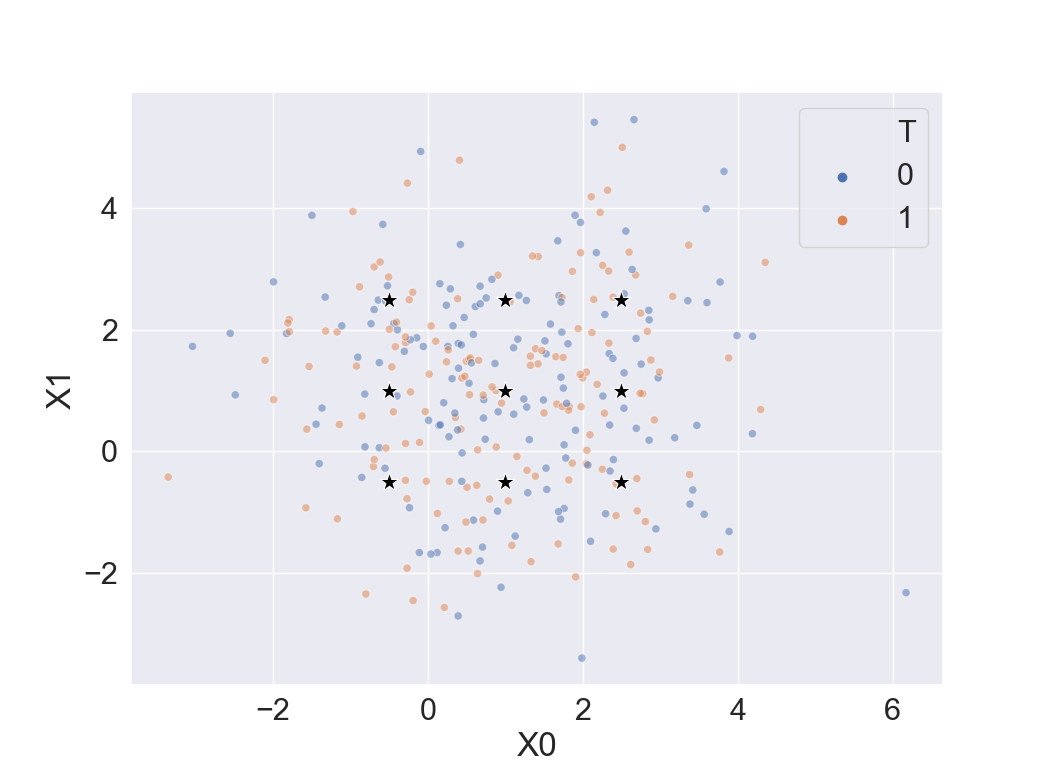
\includegraphics[width=0.7\textwidth]{Figures/coverage_space.png}\\(b)
    \caption{(a) Coverage of 95 percent confidence interval for 9 points: (1.0,1.0), (2.5,2.5), (-0.5,-0.5), (2.5,-0.5), (-0.5,2.5), (4.0,4.0), (-3.0,-3.0), (4.0,-3.0) and (-3.0,4.0). (b) Covariate space showing positions of 9 points-of-interest as black-stars, with other points color-coded according to their treatment assignments.}
    \label{fig:Coverage}
\end{figure}

Based on Figure~\ref{fig:Coverage}(a), the coverage for each the nine points of interest is between 0.9 and 1 for most of the values of variances using either of the three variance estimation approaches.

\subsection*{Limited Overlap and Performance}
We performed experiments on the overlap by changing the variance of the noise term $\epsilon_t$ in the treatment assignment equation of the DGP and measured CATE estimation error for MALTS for each of the scenarios. A lower variance leads to small overlap, i.e., large standardized difference of means, whereas large variance means small standardized difference of means and high overlap.
Figure~\ref{fig:overlap}(a) shows the performance of MALTS in predicting CATEs for 500 units in  2 dimensions generated with different levels of overlap (represented as standardized difference of means). Figure~\ref{fig:overlap}(b) shows four datasets generated with different level of overlap between the treated and control groups. MALTS performs reasonably well even under limited overlap. As expected, performance deteriorates as overlap decreases.
    \begin{figure}
        \centering
        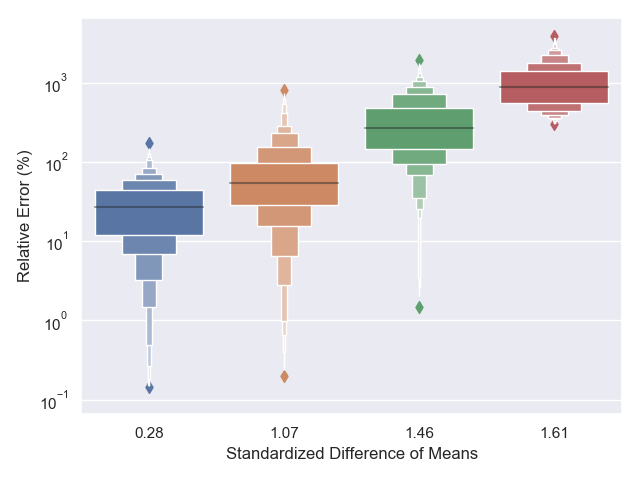
\includegraphics[width = 0.7\textwidth]{Figures/overlap.png}\\
        (a)\\
        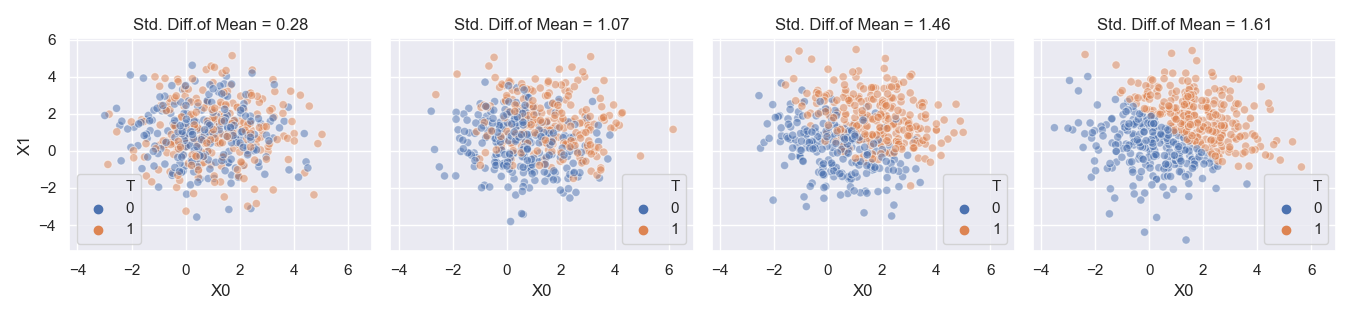
\includegraphics[width = \textwidth]{Figures/overlap_space.png}\\
        (b)
        \caption{(a) Comparison of MALTS performance measured as relative error for CATE estimation under different level of overlap measured as standardized difference of means. (b) The plots show the distribution of data generated for assessing the performance of MALTS under limited overlap.}
        \label{fig:overlap}
    \end{figure}
    
\subsection*{Sensitivity Analysis}
We performed a \textit{sensitivity analysis} of MALTS on a data generative setup with a constant unit treatment effect, two observed relevant covariates, and an unobserved confounder affecting the probability distributions of outcome as well as the choice of treatment. The unobserved confounder has a linear relationship with the outcome with the value of the coefficient equal to the ``sensitivity parameter of the Outcome'' ($\gamma_Y$) and the choice of treatment with the value of the coefficient equal to the ``sensitivity parameter of the Treatment'' ($\gamma_T$).
\begin{eqnarray*}
    && x_{i,1},x_{i,2}, u_i \overset{iid}{\sim} \mathcal{N}(0,1)\\
    && \epsilon_0, \epsilon_1 \overset{iid}{\sim} \mathcal{N}(0,1)\\
    y_i^{(0)} &=& x_{i,1} + x_{i,2} + \gamma_Y u_i + \epsilon_0 \\
    y_i^{(1)} &=& x_{i,1} + x_{i,2} + \gamma_Y u_i + 1 + \epsilon_1 \\
    t_i &=& \text{Bernoulli}\left(\text{expit}\left( x_{i,1} + x_{i,2} + \gamma_T u_i - 2 \right) \right)\\
    y_i &=& t_i(y_i^{(1)} + (1-t_i)(y_i^{(0)}
\end{eqnarray*}
Figure~\ref{fig:sensitivity} shows the contour plot of ATE estimates produced by MALTS as we change the sensitivity parameters in the data generative process. Here, the true ATE equals to 1.
    \begin{figure}
        \centering
        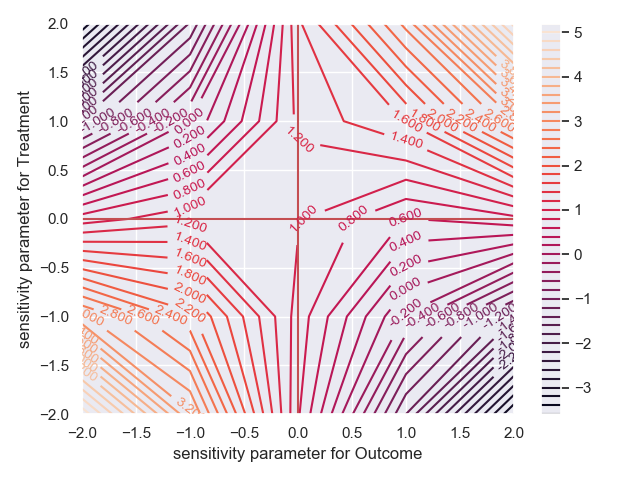
\includegraphics[width=0.85\textwidth]{Figures/sensitivity_analysis.png}
        \caption{Sensitivity analysis contour plot of the ATE estimation using MALTS}
        \label{fig:sensitivity}
    \end{figure}

    \section*{Appendix C}
In this section, we discuss our implementation of existing causal inference methods like genmatch, propensity score matching, BART, causal forest, difference of random forest,  prognostic score matching and FLAME. In Section~\ref{sec:Experiments}, we compare the performance of each of these methods with \malts.

We used MatchIt's implementation of genmatch and propensity score matching as it is commonly used by empiricists \citep{matchit2011}. We allowed matching with replacement for creating match groups and estimating CATEs. As MatchIt returns only match groups and CATE estimates for treated units (and not control units), then in order to estimate CATEs for control units, we flipped the sign of the treatment indicators and estimated negative CATEs (we have to estimate negative CATE in this case because we flipped the sign of the treatment indicator, CATE estimates became negative CATE estimates). We merged the CATE estimates for the treated units and control units to get the CATE estimates for every unit in the dataset.

We used the causal forest algorithm as implemented in the `grf' package in R. The settings for causal forest were set to the default designed by the `grf' developer with number of trees equal to $2000$ and $\sqrt{p}+20$ variables tried for each split. 

We performed the same 5-fold CATE estimation procedure for causal forest, analogous to the one used for estimating CATEs using MALTS. We estimate CATEs for both the treated and control units in each estimation set. 

We used Vincent Dorie's R implementation of BART \citep{dbart}. We performed the same 5-fold CATE estimation using BART that we used for MALTS. For each of the $\eta$ folds, we trained two BART models, one for the learning the response function for estimating the potential outcome under control and the other response function for estimating potential outcome under treatment using the training set. The CATEs were estimated by taking the difference of estimated response functions of treated and control units in the estimation set. We also implement a 5-fold FLAME CATE estimation procedure analogous to the one used by MALTS.

Lastly, we implemented 5-fold prognostic score matching using a random forest approach to model the prognostic score function. We fit a model for control units and a model for treated units using the data in the training set. To estimate the CATE for a treated unit in the estimation set, we found k-nearest neighbors in the control set with a similar estimated prognostic score. Analogously, we estimated the CATEs for the control units in the estimation set using the k-nearest treated units with similarity measured using the prognostic score.

    \section*{Appendix D}
In this section, we show the example matched group using prognostic score matching for unit id-1 in Table~\ref{tab:mg_prog} for which MALTS produces a high quality matched group, as shown in Table~\ref{tab:match-group-example}. While MALTS matches units based on a learned distance metric over the covariate space, prognostic score matching matches units based on a single prognostic value. Hence unlike MALTS, the matched group produced by prognostic score do not match closely on any of the covariates, which makes it difficult to interpret. Also there is only one point in common between the matched groups for the query between the two methods (unit 116); the matched groups are almost entirely different between the two methods.
%doesn't allow the user to analyze the results.



\begin{table}
    \caption{Example Matched Group using (a) MALTS and (b) Prognostic Score matching for query unit-id 1. The matched groups for MALTS and prognostic score are different from each other; only unit 116 is matched to the query unit for both methods, all other matched units are different.}
    \label{tab:mg_prog}
\centering
\resizebox{\textwidth}{!}{%
\begin{tabular}{lrrrrrrrrr}
\multicolumn{10}{c}{(a) MALTS}\\
\hline
\textbf{Unit-id} &
  \textbf{Treated} &
  \textbf{Age} &
  \textbf{Education} &
  \textbf{Black} &
  \textbf{Hispanic} &
  \textbf{Married} &
  \textbf{No-Degree} &
  \textbf{Income-1975} &
  \textbf{Income-1978} \\ \hline
Query-1: \textit{1}   & 1.0 & 22.0 & 9.0  & 0.0 & 1.0 & 0.0 & 1.0 & 0.0 & 3595.89  \\  \hline
\textit{94}  & 1.0 & 23.0 & 8.0  & 0.0 & 1.0 & 0.0 & 1.0 & 0.0 & 3881.28  \\
\textit{330} & 0.0 & 22.0 & 8.0  & 0.0 & 1.0 & 0.0 & 1.0 & 0.0 & 9920.94  \\
\textit{299} & 0.0 & 22.0 & 9.0  & 1.0 & 0.0 & 0.0 & 1.0 & 0.0 & 0.00     \\
\textit{5}   & 1.0 & 22.0 & 9.0  & 1.0 & 0.0 & 0.0 & 1.0 & 0.0 & 4056.49  \\
\textit{82}  & 1.0 & 21.0 & 9.0  & 1.0 & 0.0 & 0.0 & 1.0 & 0.0 & 0.00     \\
\textit{416} & 0.0 & 22.0 & 9.0  & 1.0 & 0.0 & 0.0 & 1.0 & 0.0 & 12898.38 \\
\textit{333} & 0.0 & 21.0 & 9.0  & 1.0 & 0.0 & 0.0 & 1.0 & 0.0 & 3343.22  \\
\textit{292} & 1.0 & 20.0 & 9.0  & 1.0 & 0.0 & 0.0 & 1.0 & 0.0 & 8881.67  \\
\textit{17}  & 1.0 & 23.0 & 10.0 & 1.0 & 0.0 & 0.0 & 1.0 & 0.0 & 7693.40  \\
\textit{116} & 1.0 & 24.0 & 10.0 & 1.0 & 0.0 & 0.0 & 1.0 & 0.0 & 0.00     \\ \hline
\multicolumn{10}{c}{(b) Prognostic Scores}\\
\hline
\textbf{Unit-id} &
  \textbf{Treated} &
  \textbf{Age} &
  \textbf{Education} &
  \textbf{Black} &
  \textbf{Hispanic} &
  \textbf{Married} &
  \textbf{No-Degree} &
  \textbf{Income-1975} &
  \textbf{Income-1978}\\
\hline
Query-1: \textit{1}   & 1.0 & 22.0 & 9.0  & 0.0 & 1.0 & 0.0 & 1.0 & 0.0 & 3595.89  \\  \hline
154 &    1.0 &  22.0 &       10.0 &    1.0 &       0.0 &      0.0 &       1.0 &   1071.10 &  7315.45 \\
56  &    1.0 &  30.0 &       11.0 &    1.0 &       0.0 &      1.0 &       1.0 &      0.00 &   590.78 \\
100 &    1.0 &  17.0 &       10.0 &    1.0 &       0.0 &      0.0 &       1.0 &      0.00 &     0.00 \\
109 &    1.0 &  18.0 &        9.0 &    1.0 &       0.0 &      0.0 &       1.0 &      0.00 &  4482.84 \\
141 &    1.0 &  25.0 &        8.0 &    1.0 &       0.0 &      0.0 &       1.0 &  37431.66 &  2346.82 \\
286 &    1.0 &  23.0 &       12.0 &    0.0 &       1.0 &      0.0 &       0.0 &   1117.43 &   559.44 \\
338 &    0.0 &  44.0 &        9.0 &    1.0 &       0.0 &      0.0 &       1.0 &      0.00 &  9722.00 \\
340 &    0.0 &  22.0 &       12.0 &    1.0 &       0.0 &      0.0 &       0.0 &    532.25 &  1333.44 \\
355 &    0.0 &  18.0 &       10.0 &    0.0 &       1.0 &      0.0 &       1.0 &      0.00 &  1859.16 \\
116 &    1.0 &  24.0 &       10.0 &    1.0 &       0.0 &      0.0 &       1.0 &      0.00 &     0.00 \\
\hline
\end{tabular}
}

\end{table}

\end{document}